\subsubsection{User registration}
Each individual should register an account in order to use the System. The user initially fills a form on its smartphone providing all the required data. The Mobile App also collects the model of the smartwatch. \\
This data is sent over the internet, using an HTTP POST request to the AuthenticationManager, with all the required data in JSON format. The AuthenticationManager firstly checks if the smartatch is compatible. If it is, it checks that the email and SSN/fiscal code are not used by any individual already registered. If all the check pass an Individual and an Account are created in the database.\\
The account initially is not confirmed.\\
Then, a mail is sent to the email provided, with a verification code.
When the user inserts the verification code in the app, an HTTP POST request is made to the System and the user, if the code is correct, is put in the active state.
\begin{figure}[H]
	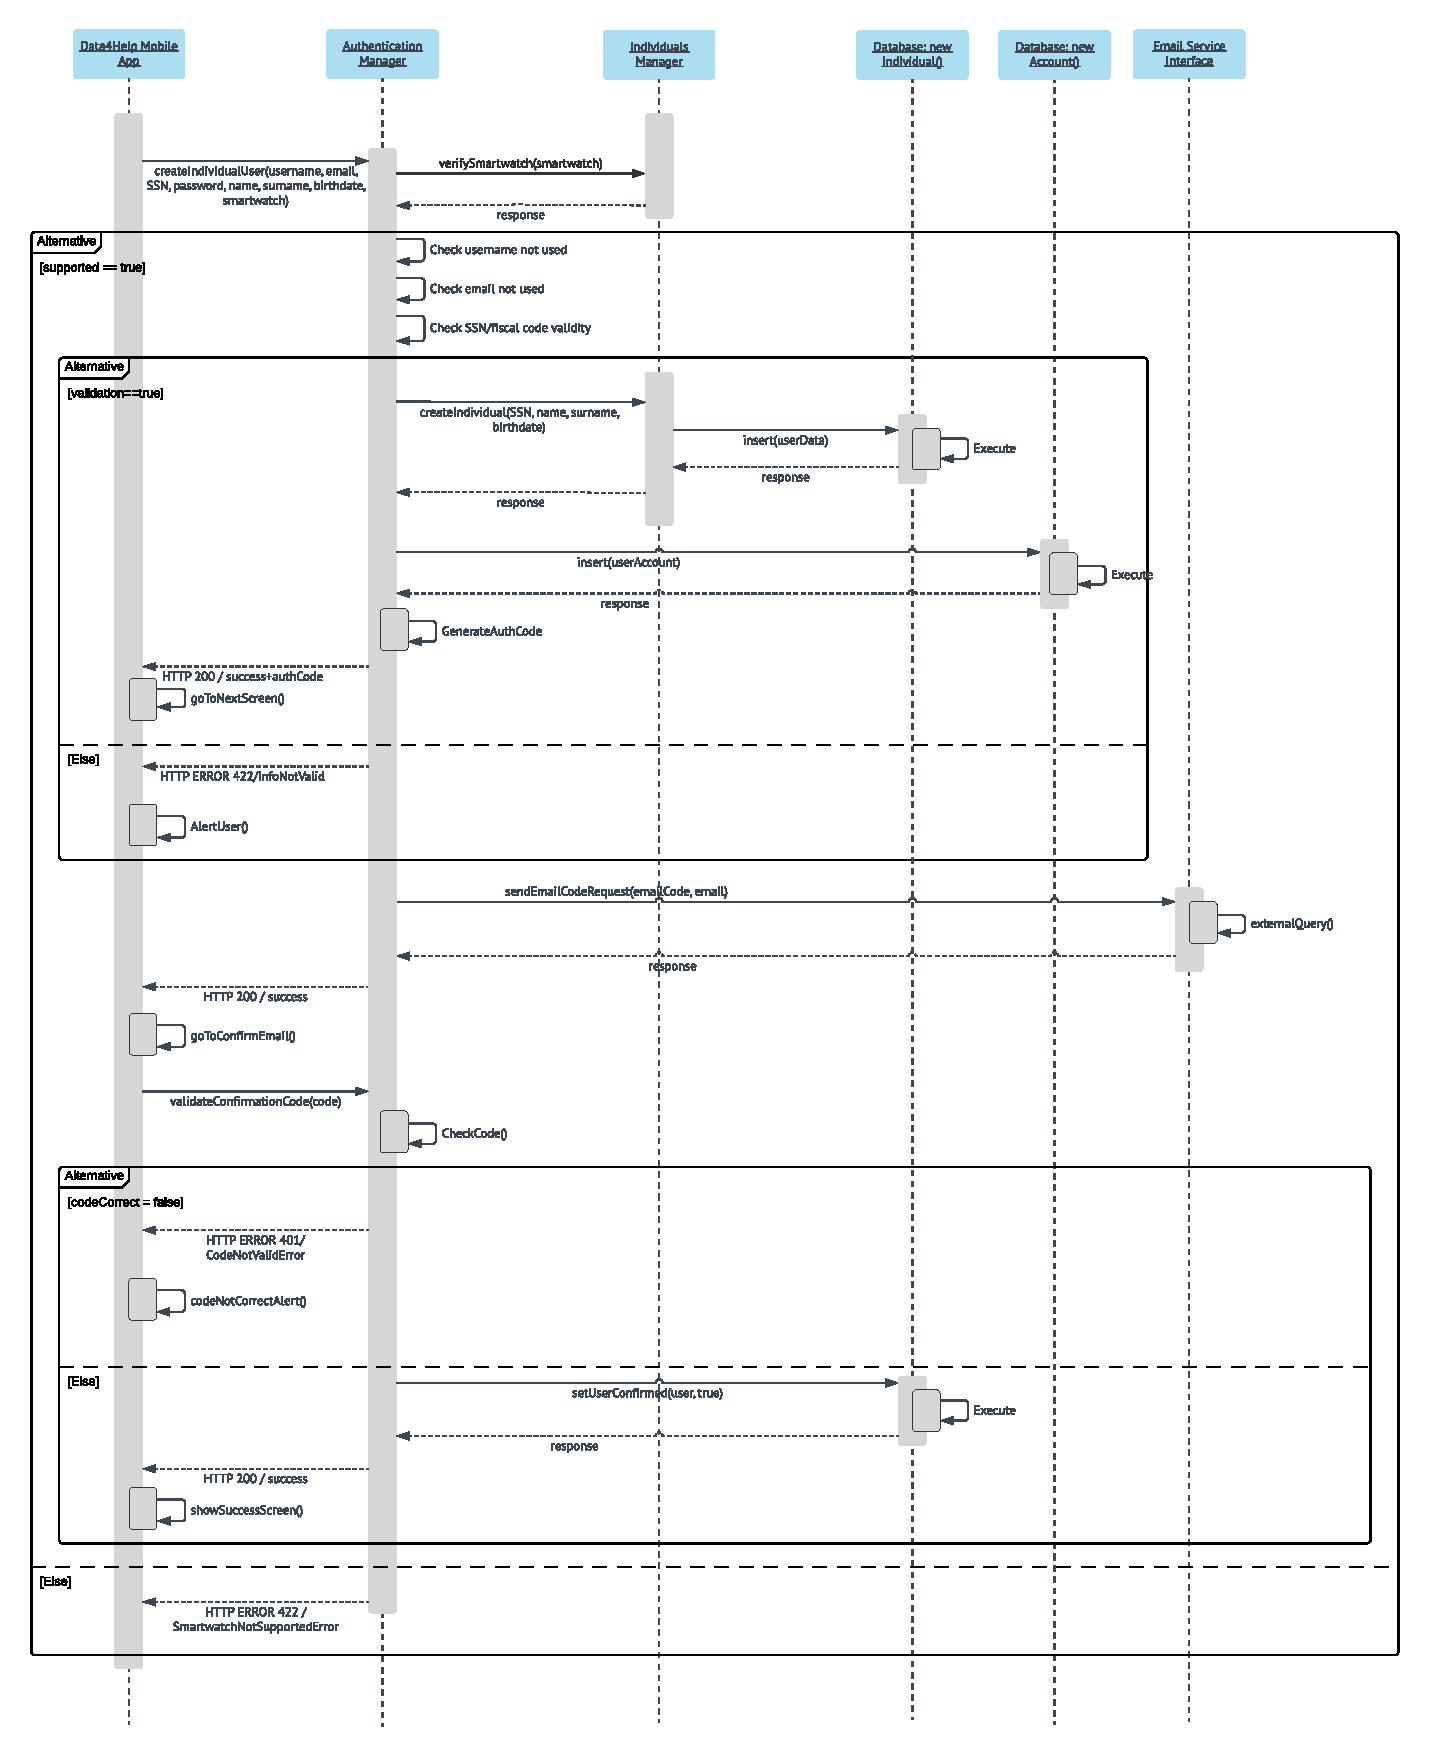
\includegraphics[width=\textwidth,height=\textheight,keepaspectratio]{assets/flowCharts/IndividualRegistration.pdf}
	\caption{User registration Runtime View}
	\label{fig:IndividualRegistration}
\end{figure}


\subsubsection{General Login}
When a generic user (one among Individual, Company or Run organizer) wants to login, an HTTP POST request is made to the authentication manager. It checks if the username and password combination are correct.\\
If they are, it generates an authToken, stores it in the database and then returns it to the caller.
The caller can use this authentication token for each subsequent call; the token will remain valid for 24 hours.
\begin{figure}[H]
	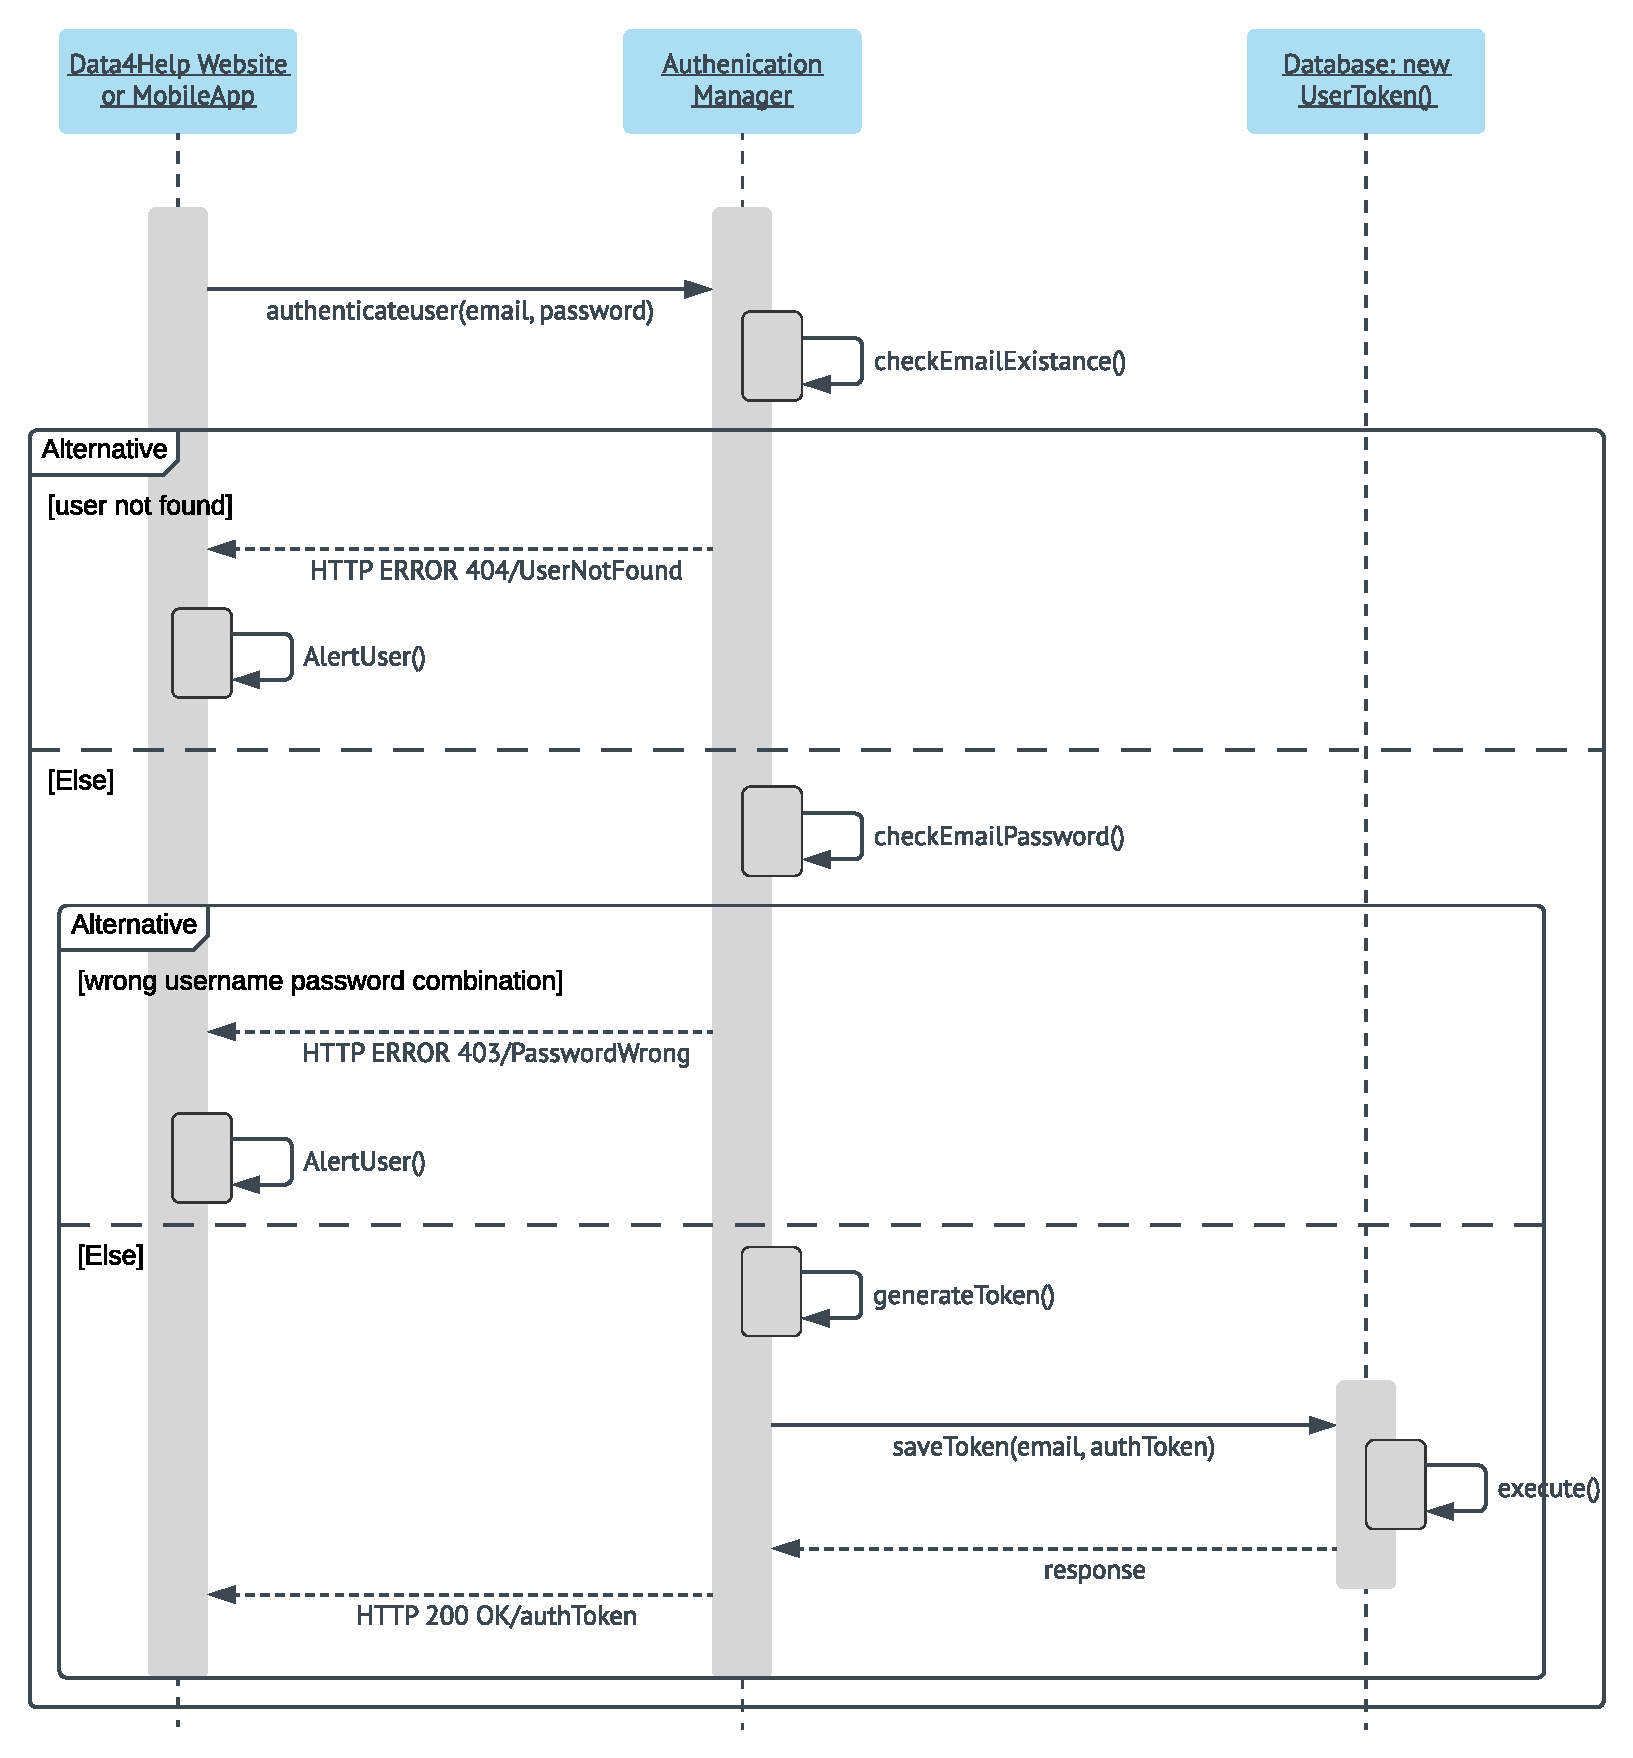
\includegraphics[width=\textwidth,height=\textheight,keepaspectratio]{assets/flowCharts/UserLogsIn.pdf}
	\caption{General Login Runtime View}
	\label{fig:UserLogsIn}
\end{figure}



\subsubsection{Consulting Individual Activity History}
When an Individual wants to look at its activity history, the app makes an HTTP GET request to the IndividualManager, including, beside the auth code, the begin date, the end date and the parameter type that he wants to get. \\
After checking the token, the IndividualManager gets the SSN and then looks for the data requested in the database. Then it returns the data found to the caller.
\begin{figure}[H]
	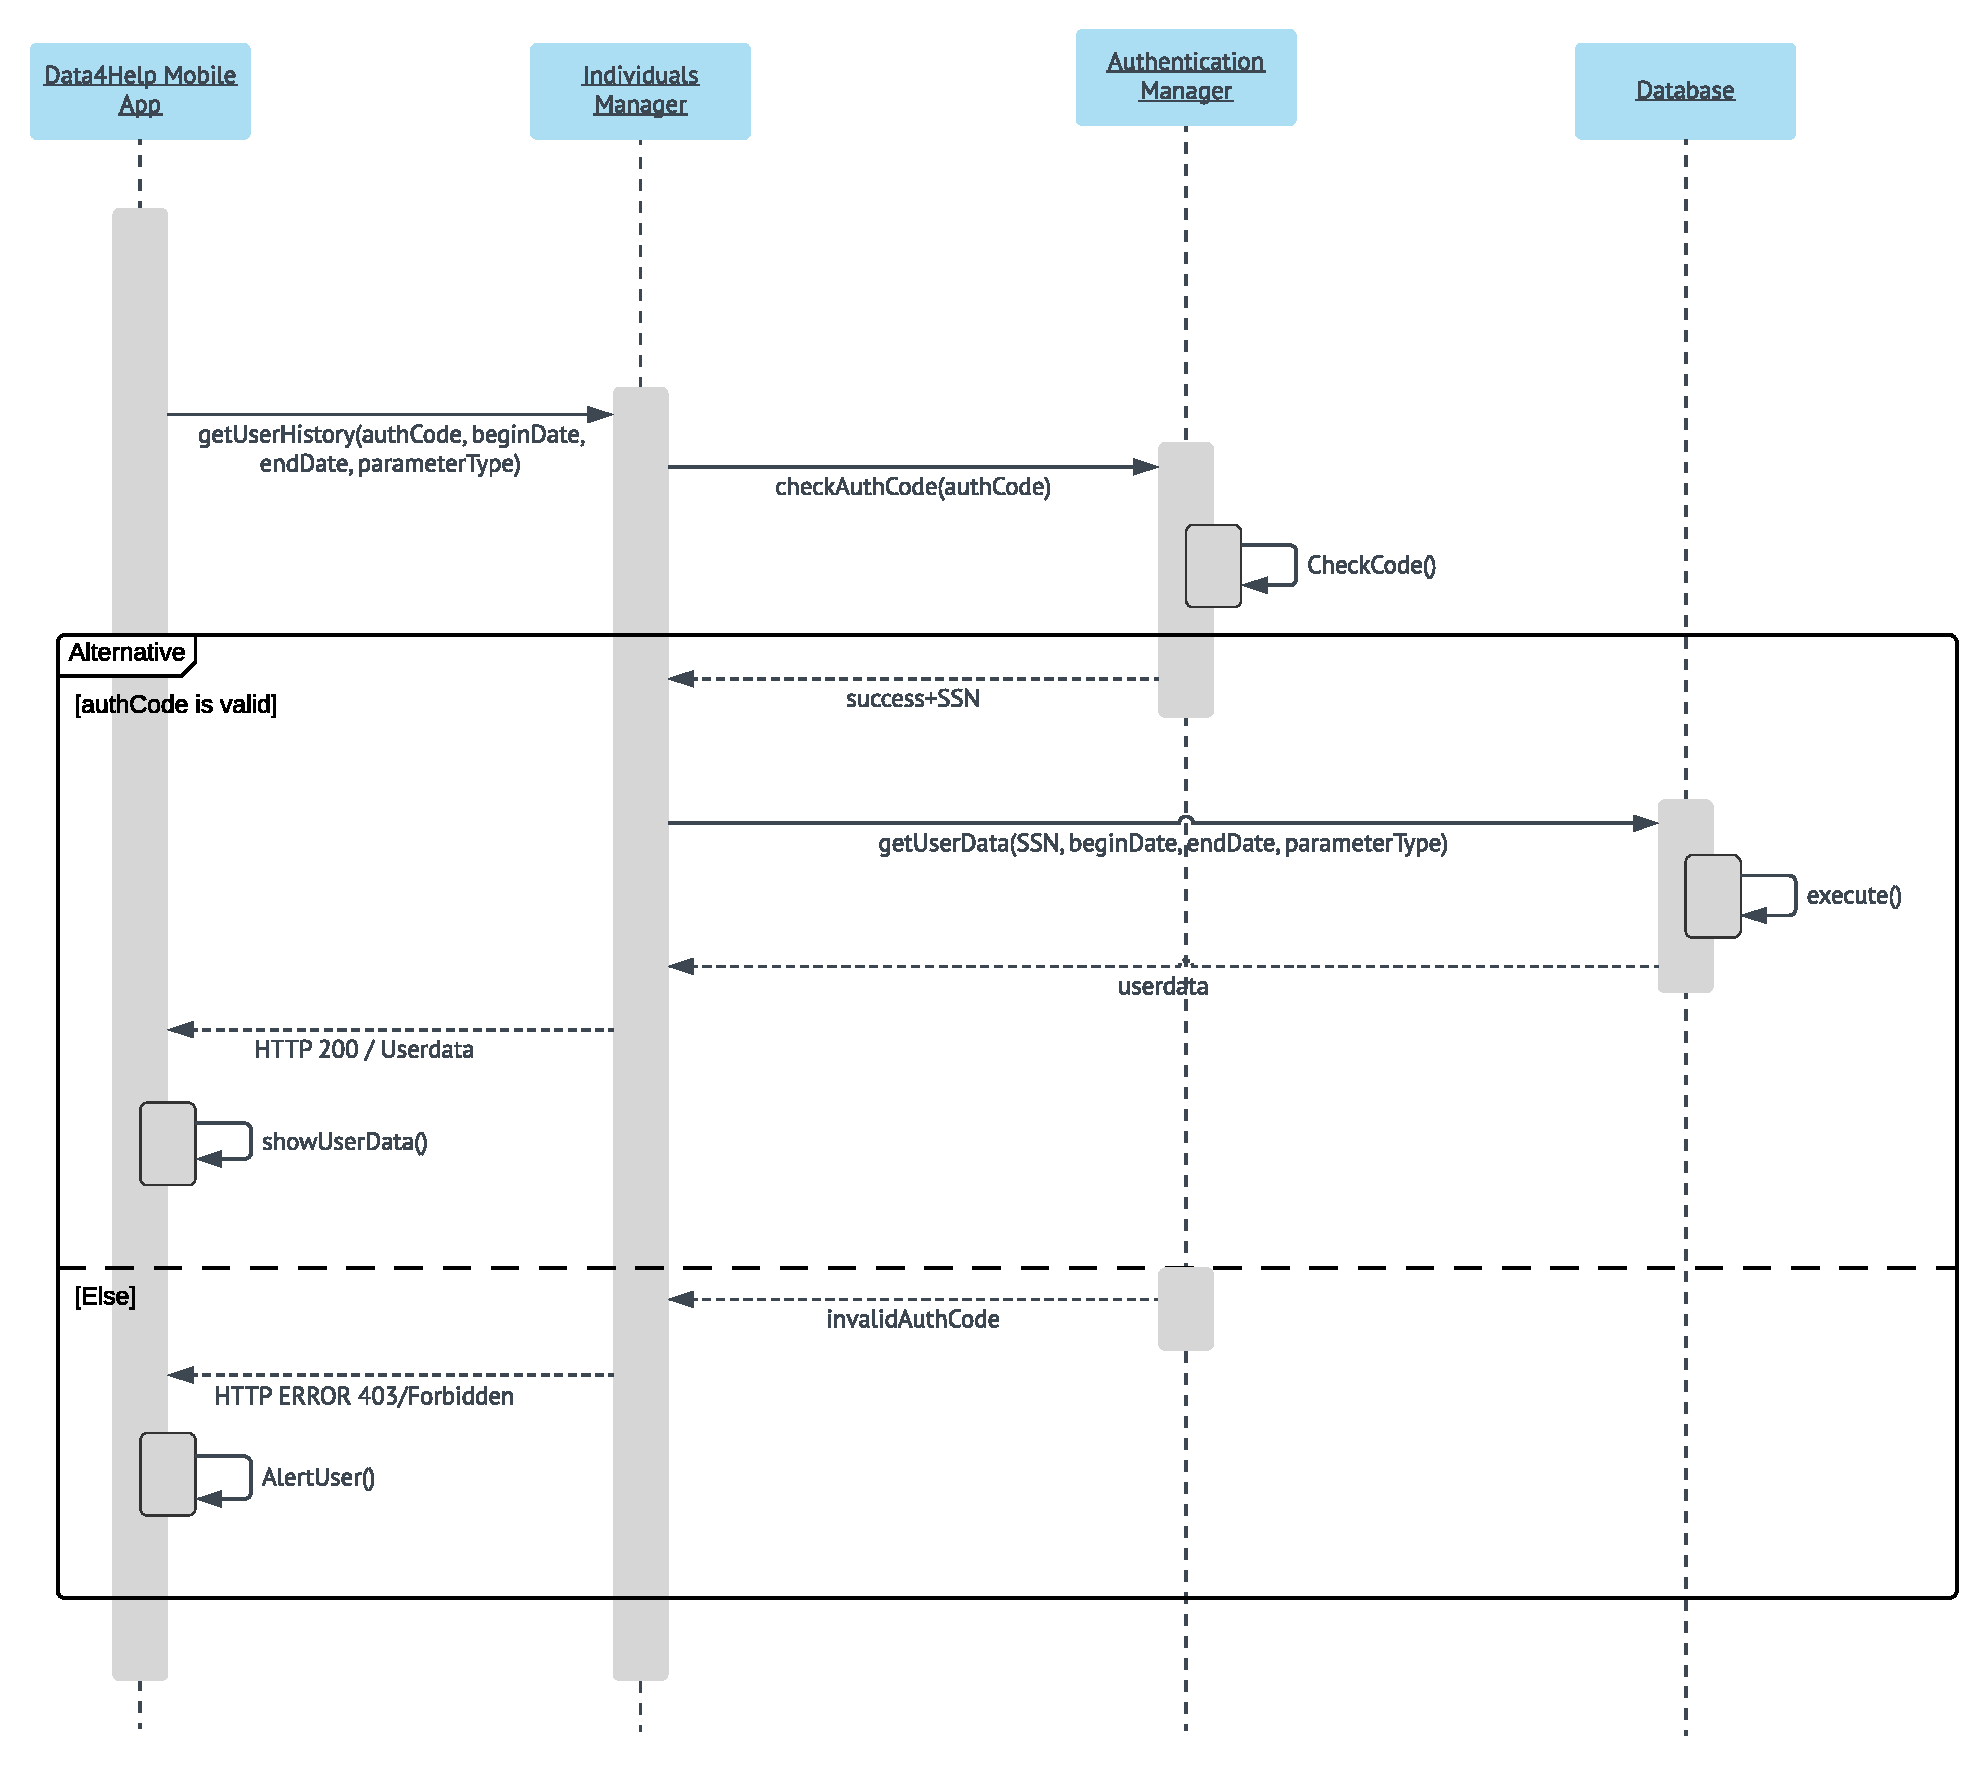
\includegraphics[width=\textwidth,height=\textheight,keepaspectratio]{assets/flowCharts/ConsultingIndividualActivityHistory.pdf}
	\caption{Consulting Individual Activity History Runtime View}
	\label{fig:ConsultingIndividualActivityHistory}
\end{figure}

\subsubsection{Data Synchronization}
When the bluetooth is activated, the Mobile App tries to enstabilish a connection with the Smartwatch App. When the connection is enstabilished, the Mobile App tries to get new data from the Smartwatch. If there is new data, it gets it and send it to IndividualManager through an HTTP POST request, alongside with the authToken perviously obtained. If the authToken is correct, the IndividualManager saves the data and then makes a call to checkUserTreshold in EmergencyManager and notifyCompanies in QueryManager.
\begin{figure}[H]
	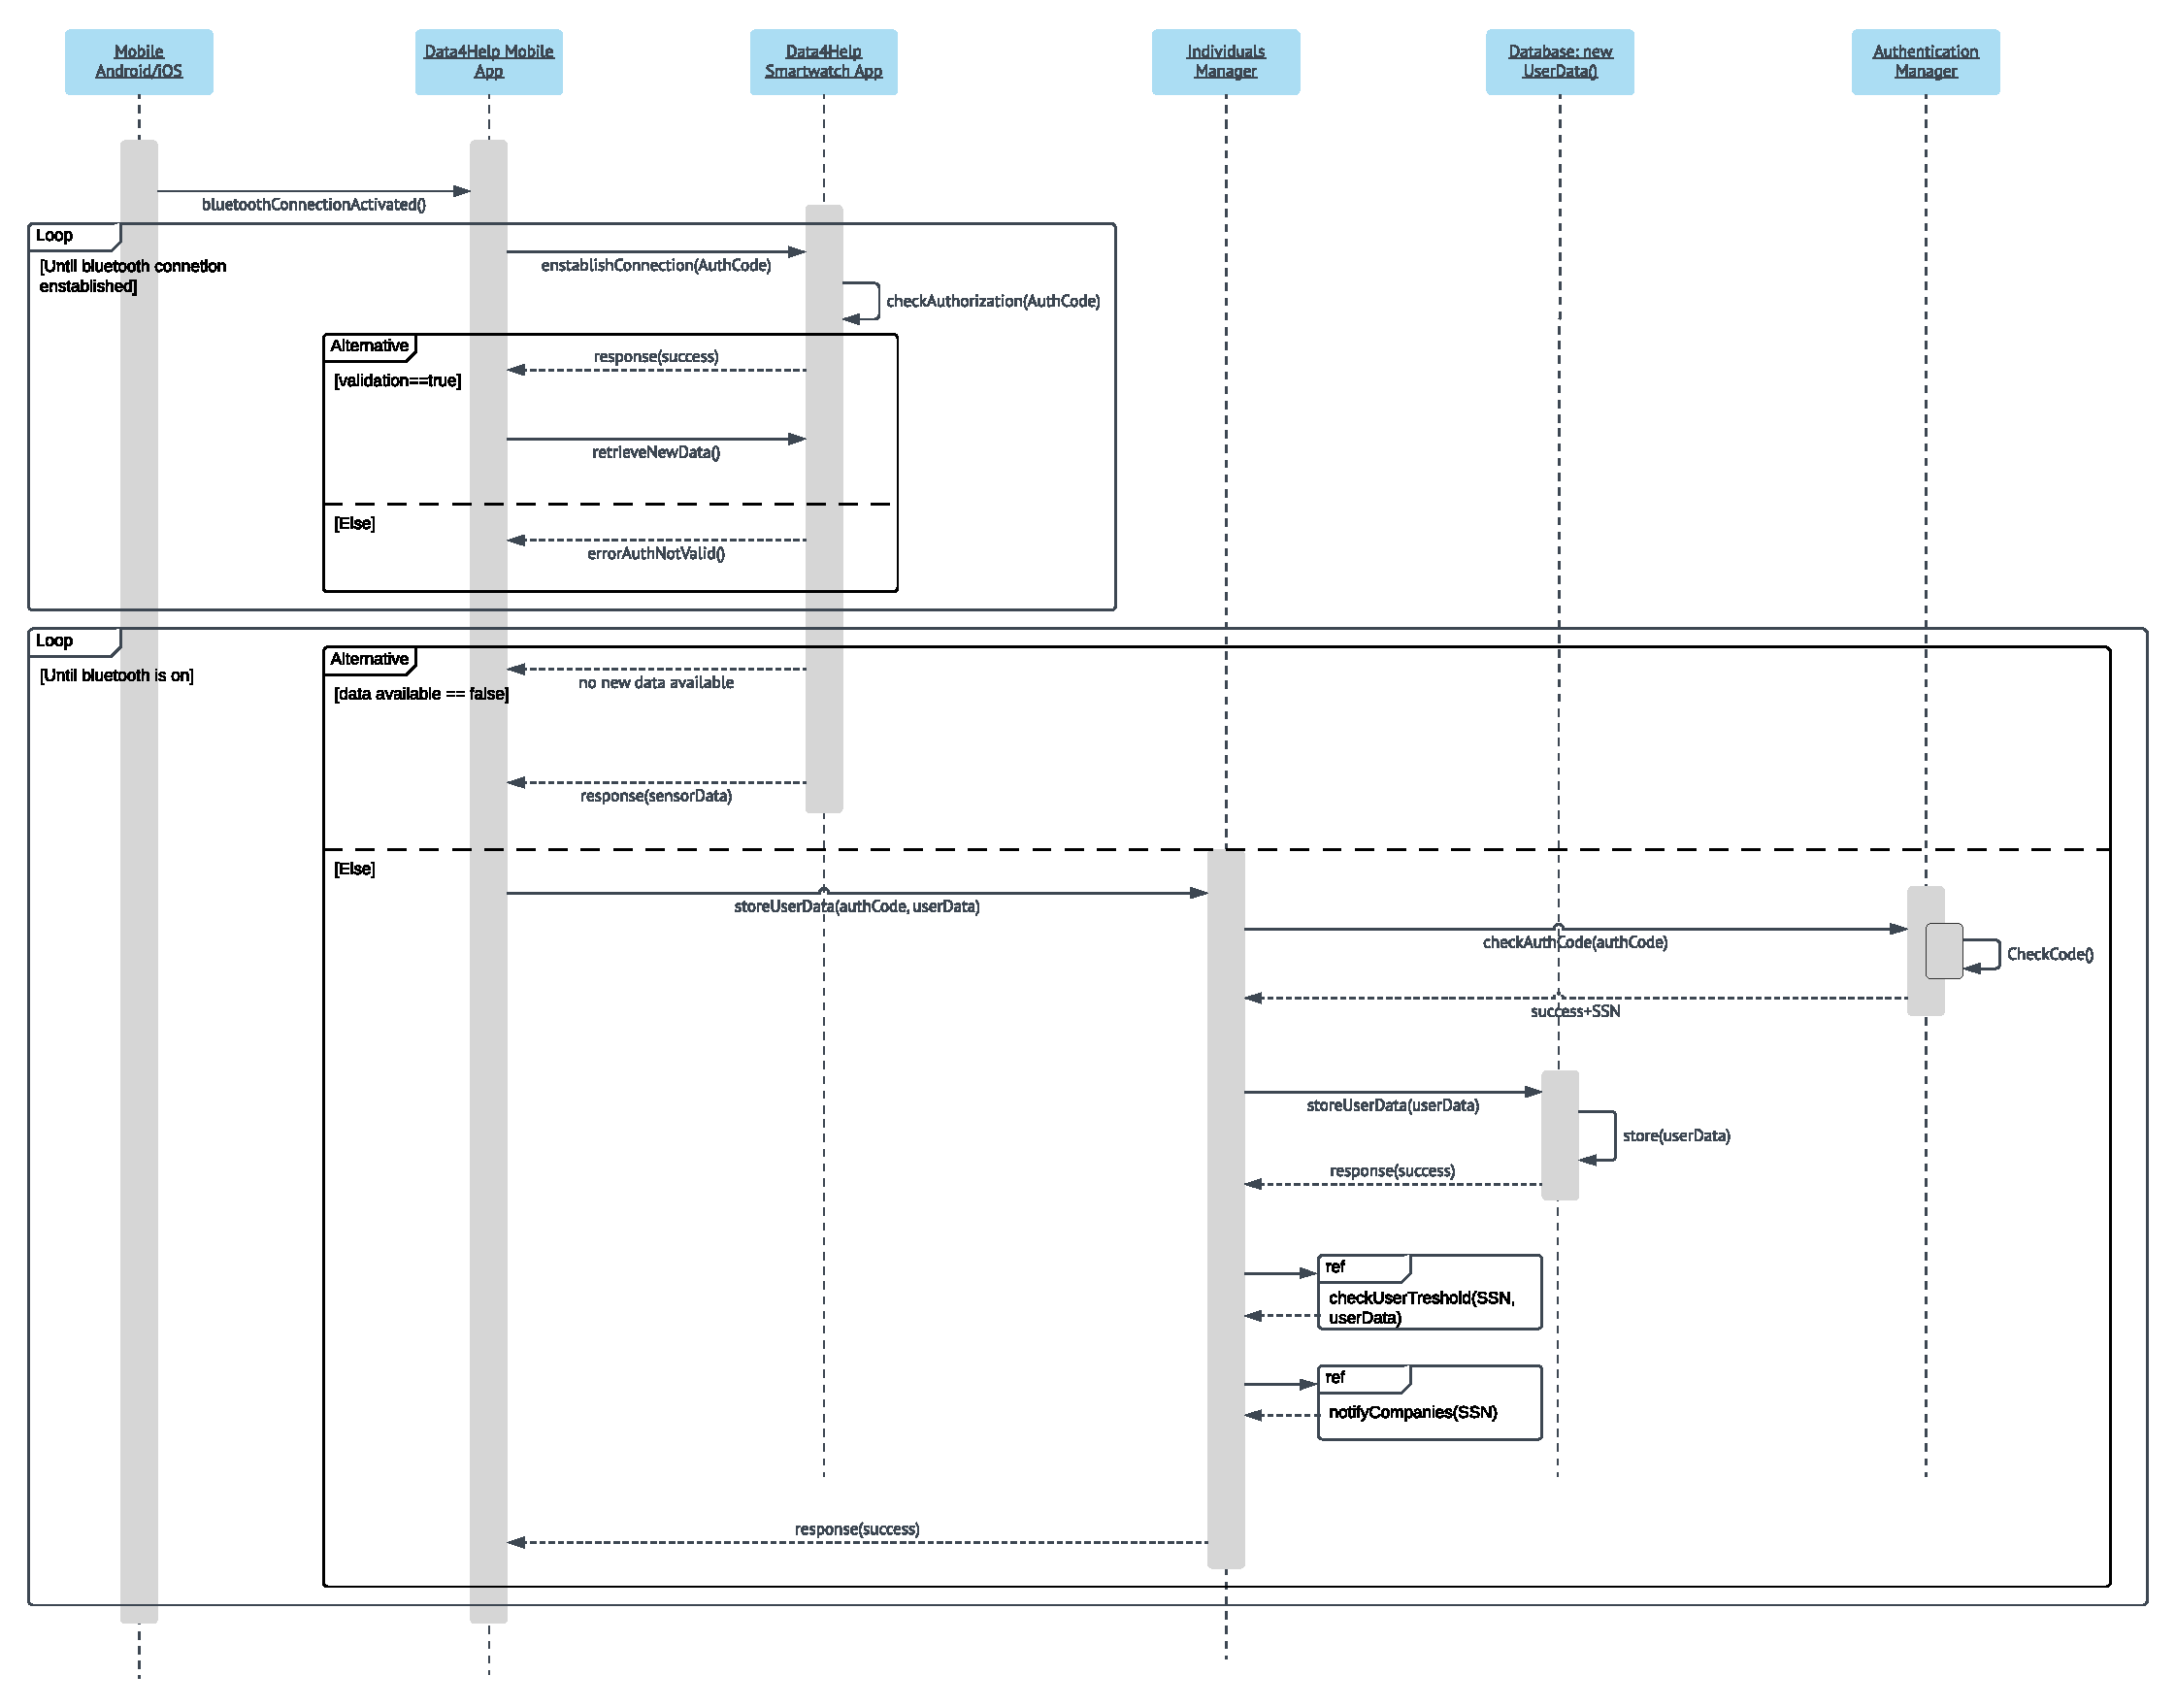
\includegraphics[width=\textwidth,height=\textheight,keepaspectratio]{assets/flowCharts/DataSynchronizationSmartwatchSmartphone.pdf}
	\caption{Data Synchronization Runtime View}
	\label{fig:DataSynchronizationSmartwatchSmartphone}
\end{figure}

\subsubsection{Company Registration}
The flow is the same as per the user regstration, excluding that the smartwatch is not checked and the user is only created in the AuthenticationManager database.
\begin{figure}[H]
	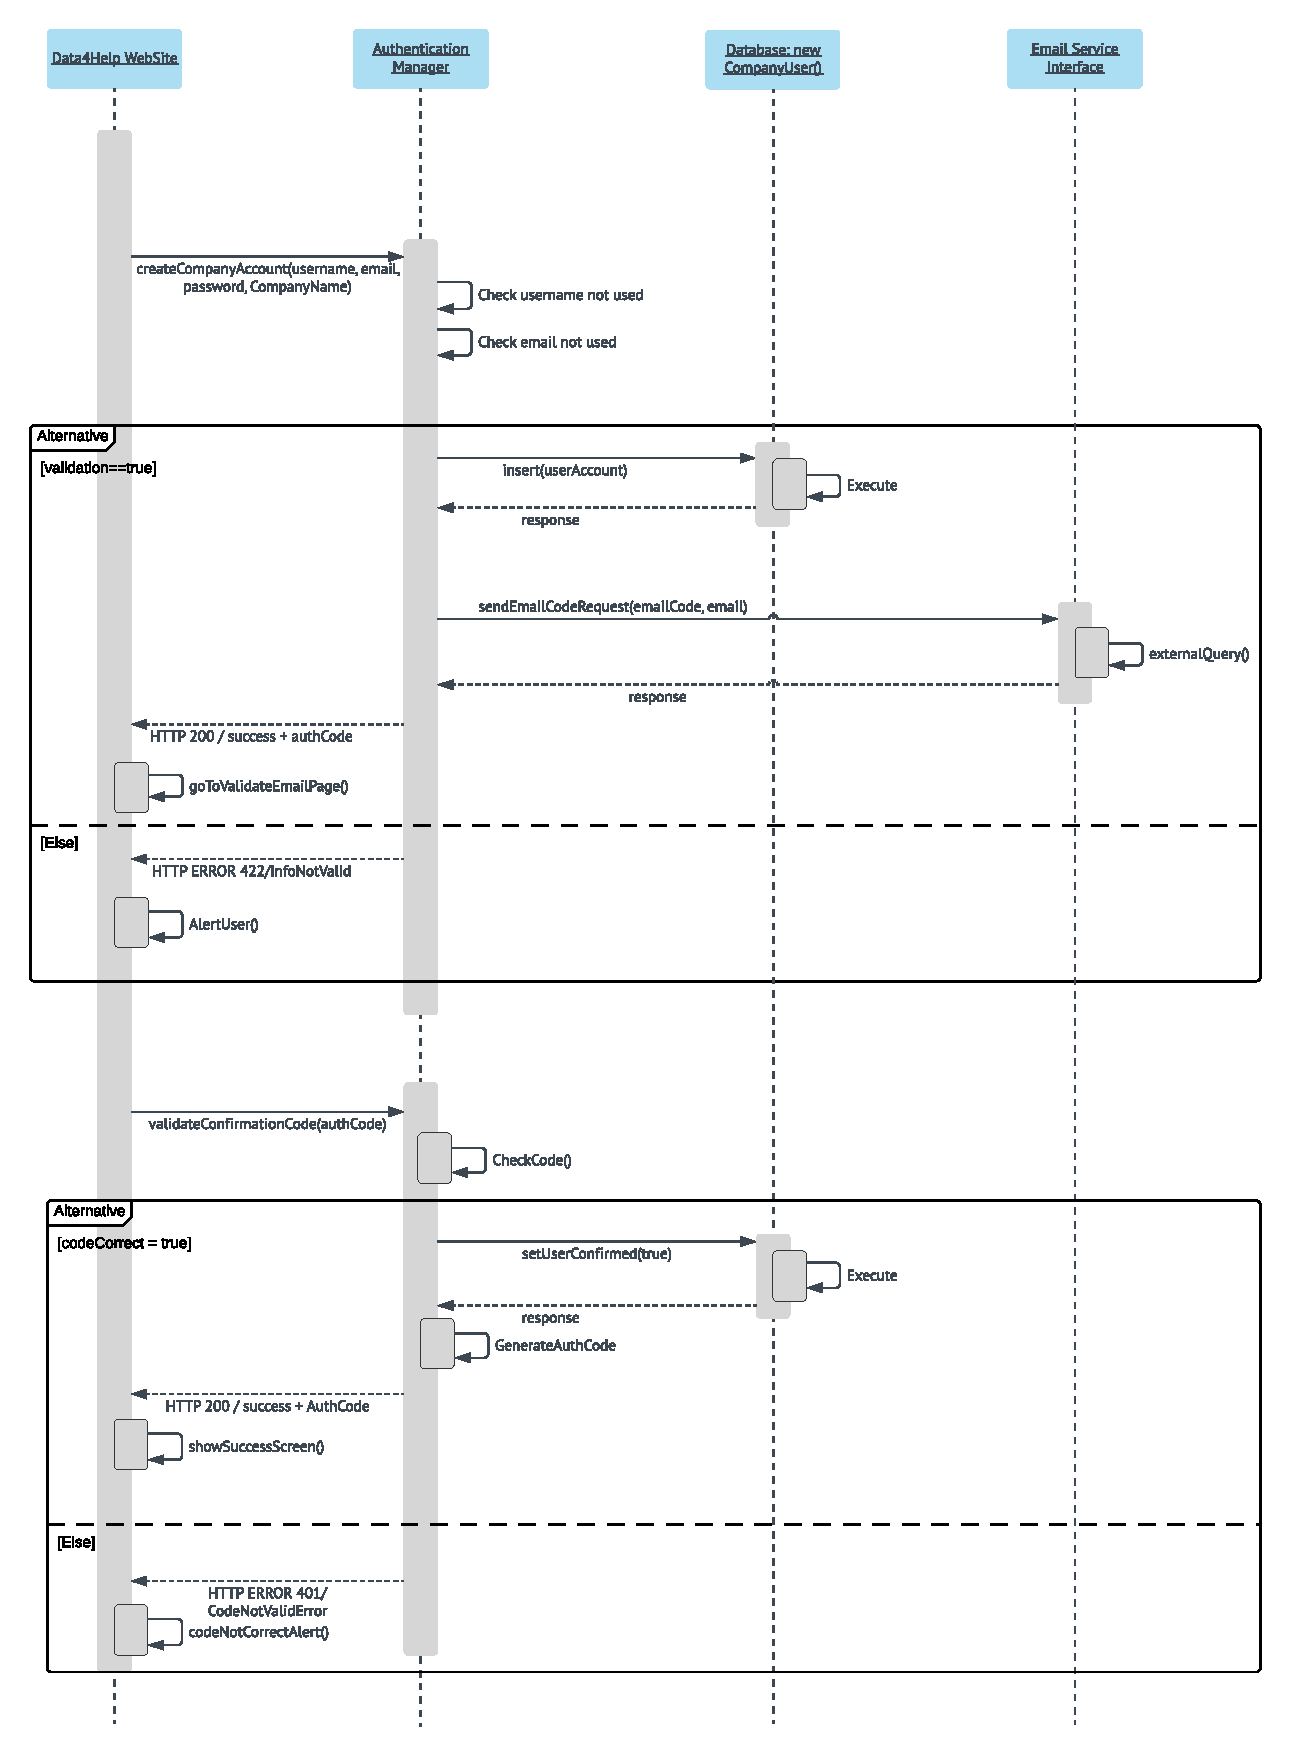
\includegraphics[width=\textwidth,height=\textheight,keepaspectratio]{assets/flowCharts/CompanyRegistration.pdf}
	\caption{Company Registration Runtime View}
	\label{fig:CompanyRegistration}
\end{figure}

\subsubsection{Company Query Search Multiple Individuals}
When a Company wants to make a query over an anonymized group of people, it accesses to the website and starts a query. The Website makes an HTTP GET request to the query manager that, after the usual security check on the authToken, checks with the help of the SubscriptionManager if the company has a plan active that allows it to make this type of query, and return the result.\\
The Company fills the form and then the Website submits it via an HTTP POST request to the Query manager with the query parameters. The QueryManager checks again the subscription and after that it compute the number of user involved in the query. If the number is below the treshold (1000) the query is blocked and an error is returned. Otherwise, the query is saved and the OK result is returned.\\
If the user then wants to download the query result, it can invoke the downloadData method on the Query manager that, after having checked the authorization, returns an XML file containing the result of the query.

\begin{figure}[H]

	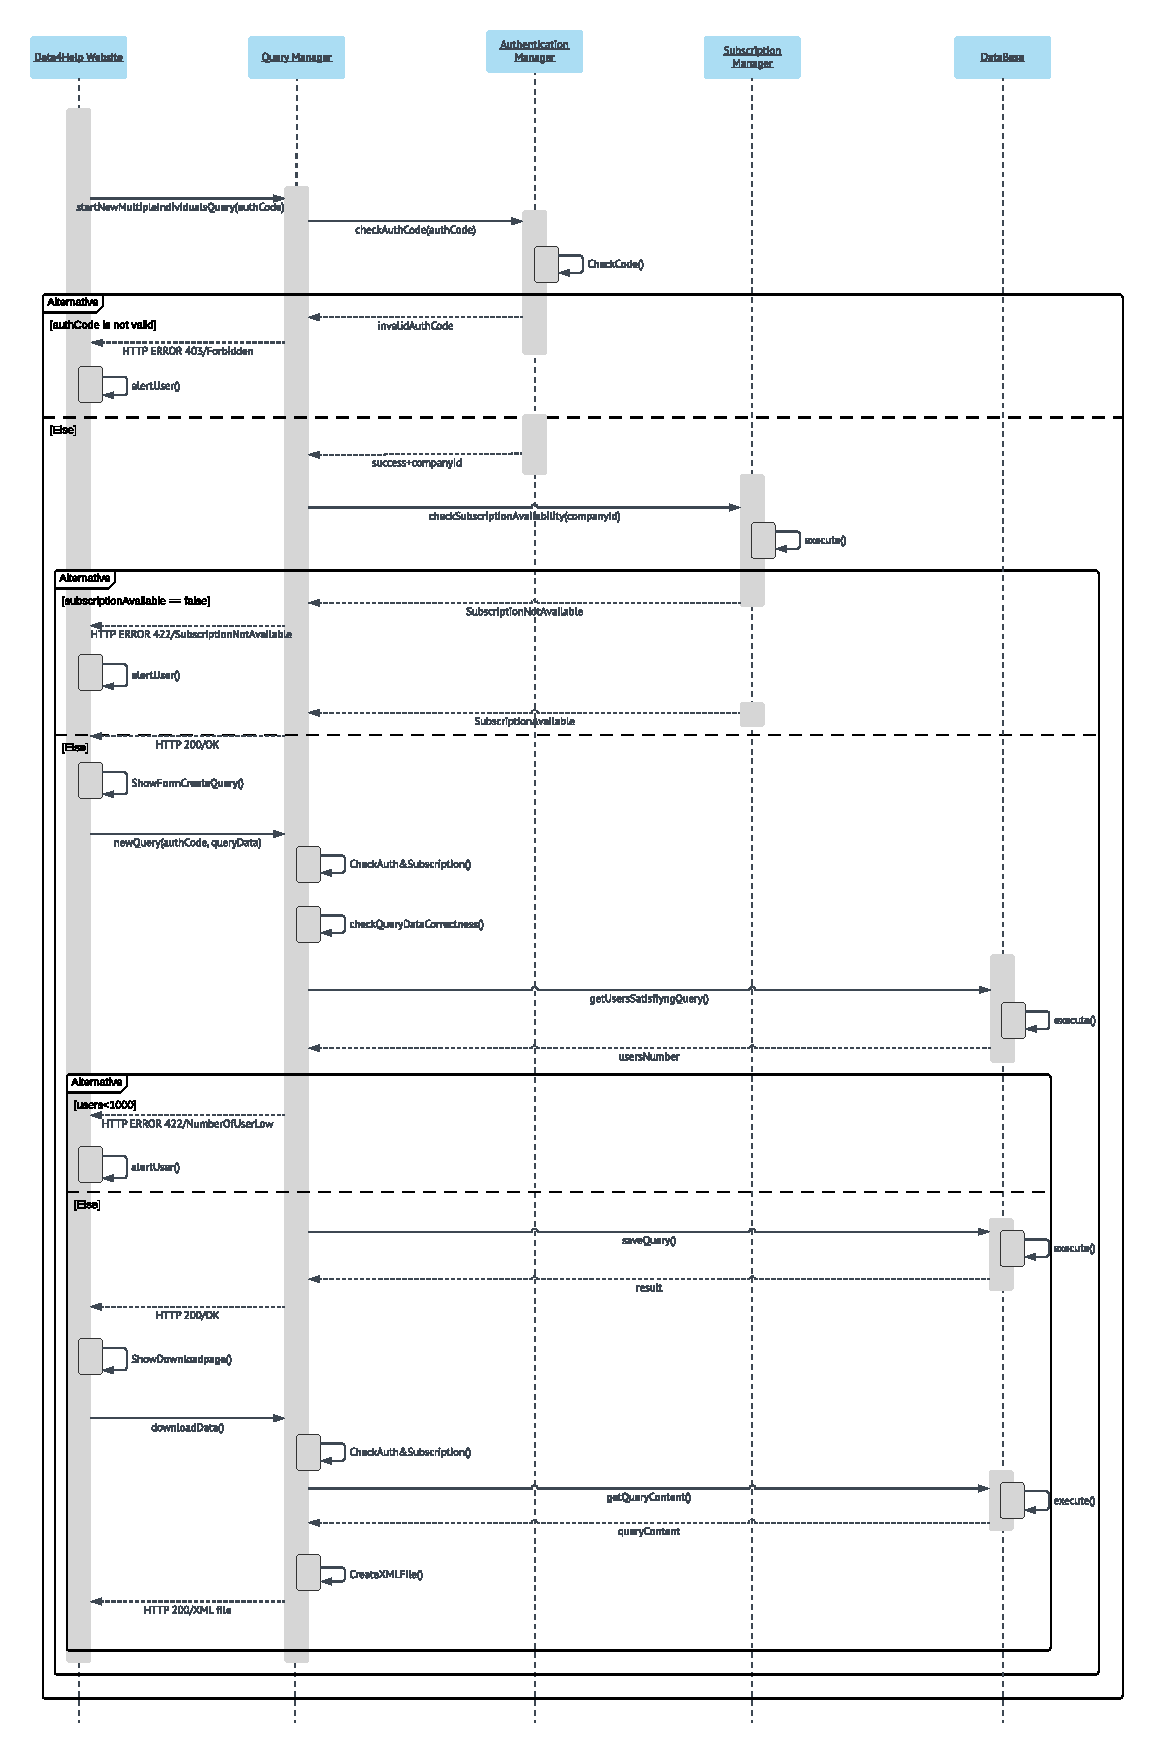
\includegraphics[width=\textwidth,height=\textheight,keepaspectratio]{assets/flowCharts/CompanyQuerySearchMultipleIndividuals.pdf}
	\caption{Company Query Search Multiple Individuals Runtime View}
	\label{fig:CompanyQuerySearchMultipleIndividuals}
\end{figure}

\subsubsection{Company Request Individual Monitoring}
When a Company wants to monitor a single user, it must ask trough the website the permission to the user.\\
The Website sends an HTTP POST request specifiyng the SSN/Fiscal code to monitor to the query manager, that, after checking the correctness of the authToken and obtained the CompanyId, checks with the help of the SubscriptionManager if the company has a plan active that allows it to make this type of query. (omitted from the graph for the sake of readability)\\
If the check passes, a new individual with the state noDecision is inserted in the Database.\\
Then, a notification is sent to the Mobile App instance of the user whose SSN is the object of the query.\\
When the user receives the notification it can either accept it or refuse it. After the click an HTTP POST request is made to the query manager and the query state is updated accordingly.

\begin{figure}[H]
	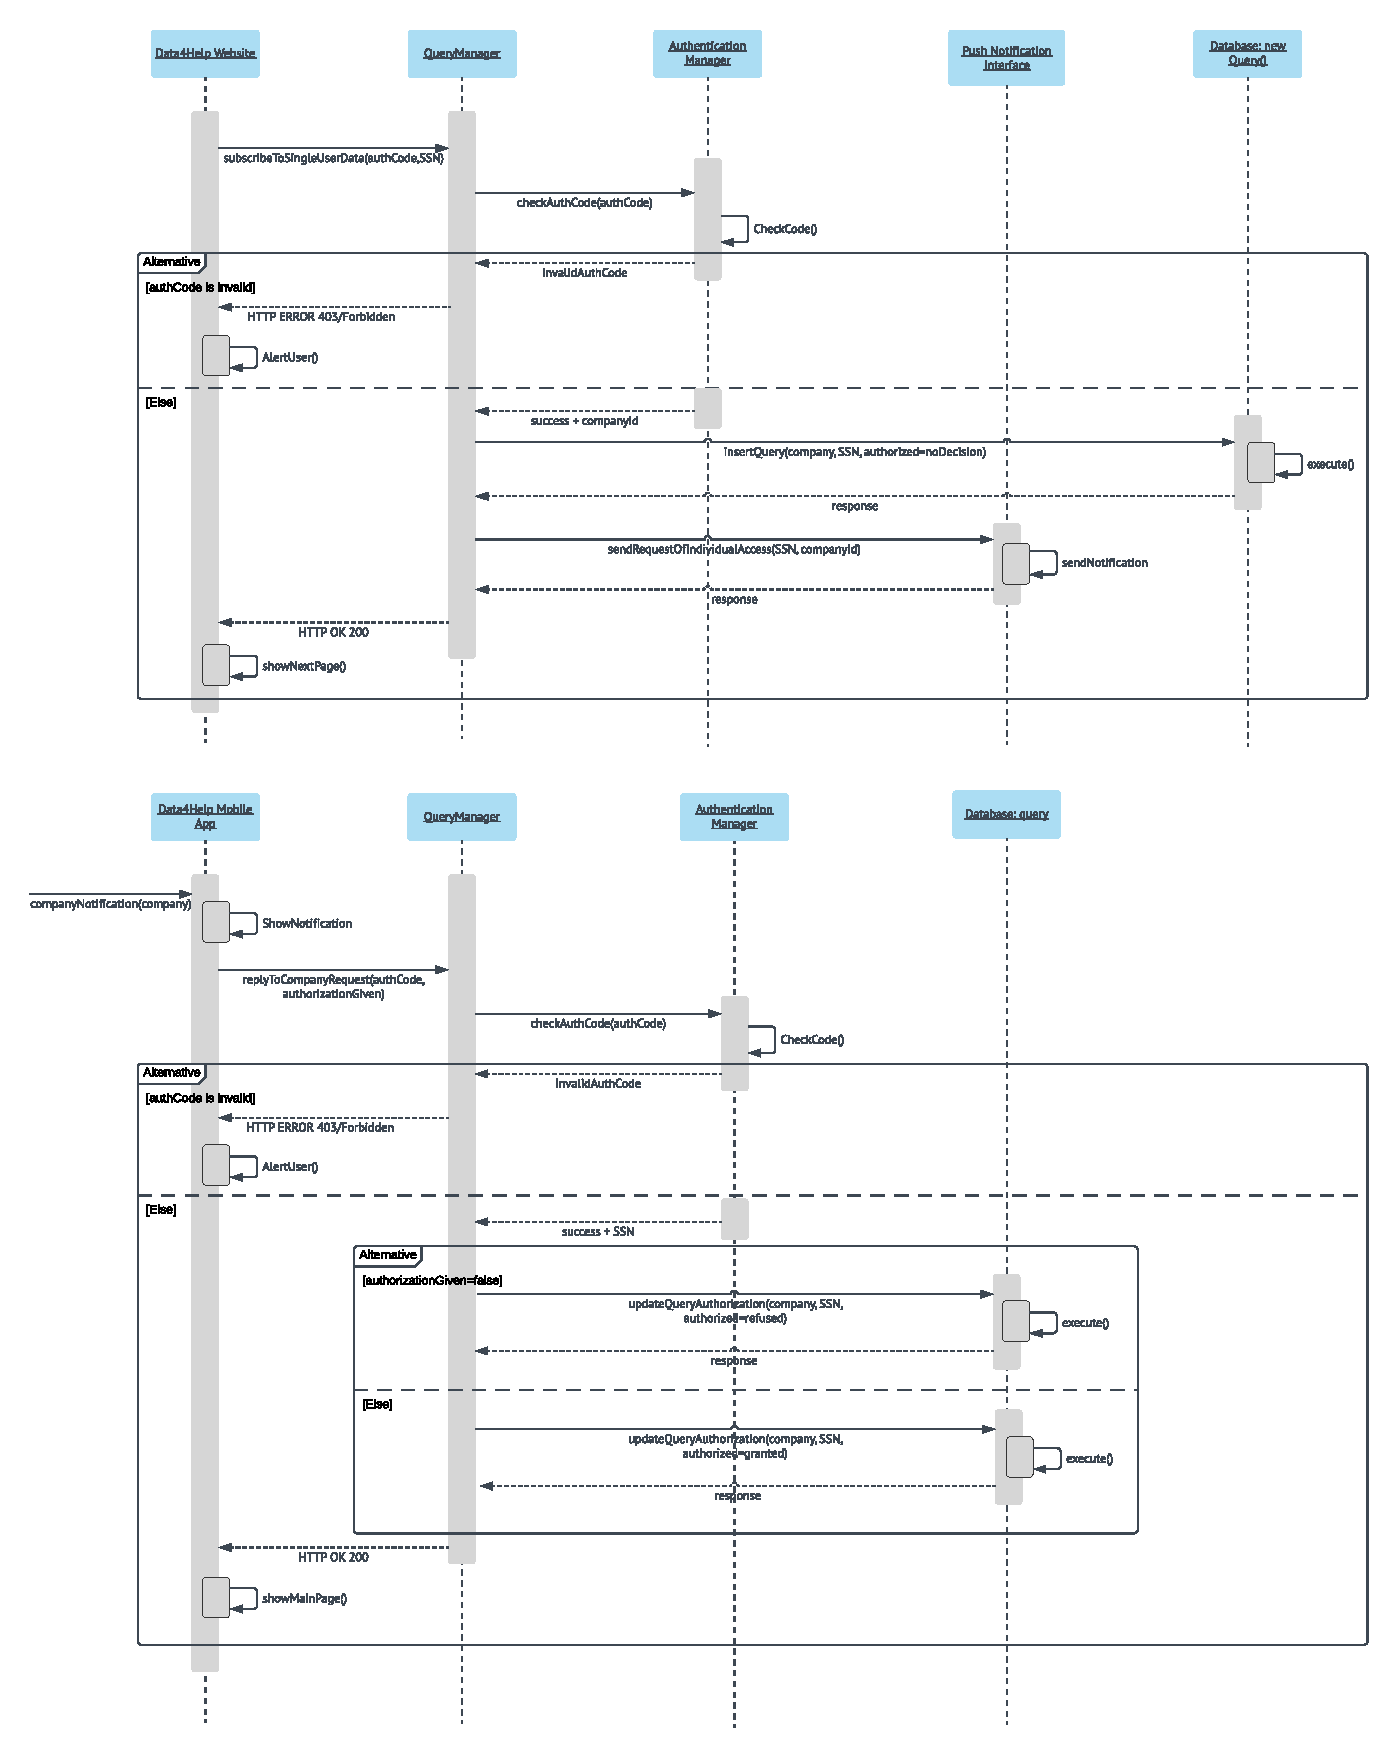
\includegraphics[width=\textwidth,height=\textheight,keepaspectratio]{assets/flowCharts/CompanyRequestIndividualMonitoring.pdf}
	\caption{Company Request Individual Monitoring Runtime View}
	\label{fig:CompanyRequestIndividualMonitoring}
\end{figure}

\subsubsection{Company Consulting Individual}
When a company wants to see an Individual's historical data, through the website, it makes an HTTP GET request to the QueryManager, specifying the SSN, the parameter type and the starting and ending date. The query manager checks the authToken, retrives the companyId and checks if the Company still has a valid plan to make this type of request. If that's indeed the case, the QueryManager checks if the Individual has given Company the authorization to see its data. If this is the case, the user data is retrieved and returned.
\begin{figure}[H]
	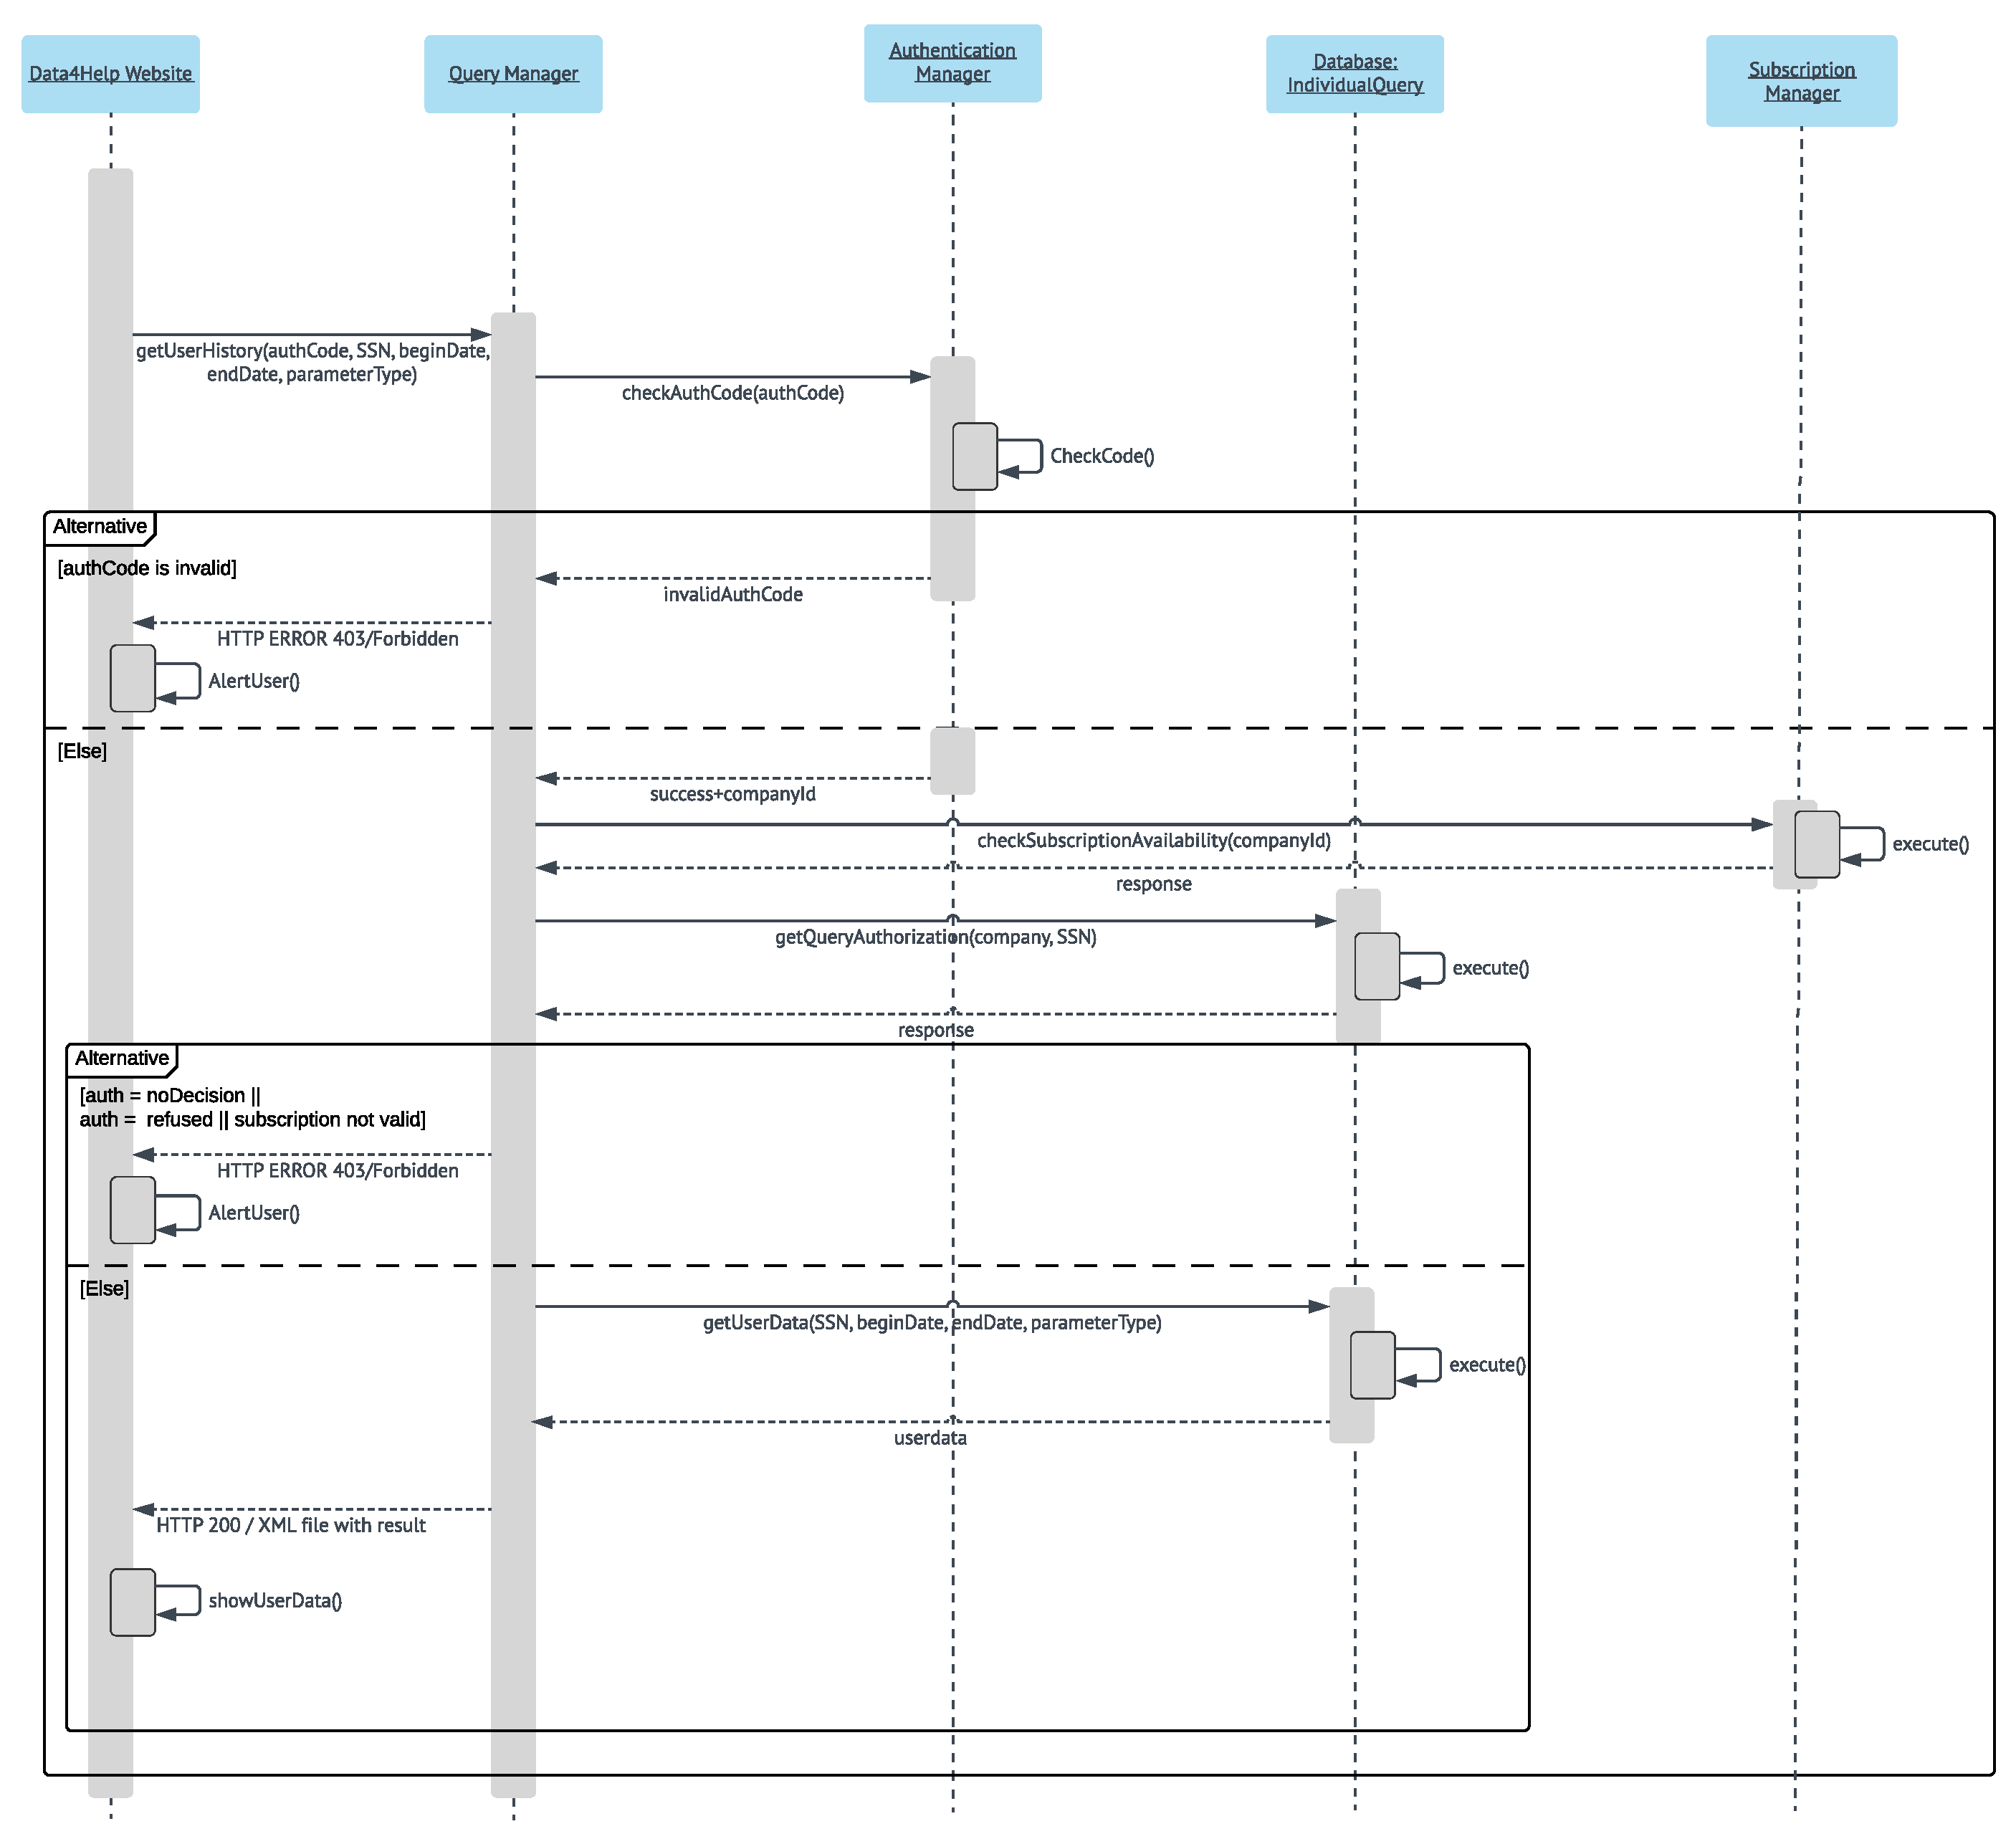
\includegraphics[width=\textwidth,height=\textheight,keepaspectratio]{assets/flowCharts/CompanyConsultingIndividualData.pdf}
	\caption{Company Consulting Individual Data Runtime View}
	\label{fig:CompanyConsultingIndividualData}
\end{figure}

\subsubsection{Company Payment Processing}
When a Company wants to buy a subscription plan, it activates the corresponding functionality in the Website, selects the subscriptionType and insert the credit card number and the CCV/Security code. This data is sent to the server through a HTTP POST request to the SubscriptionManager. After checking the authToken and retrieved the companyId, a call is made to the PaymentInterface to process the payment. If the payment is successfull, the subscription is inserted in the Database and linked to the company.
\begin{figure}[H]
	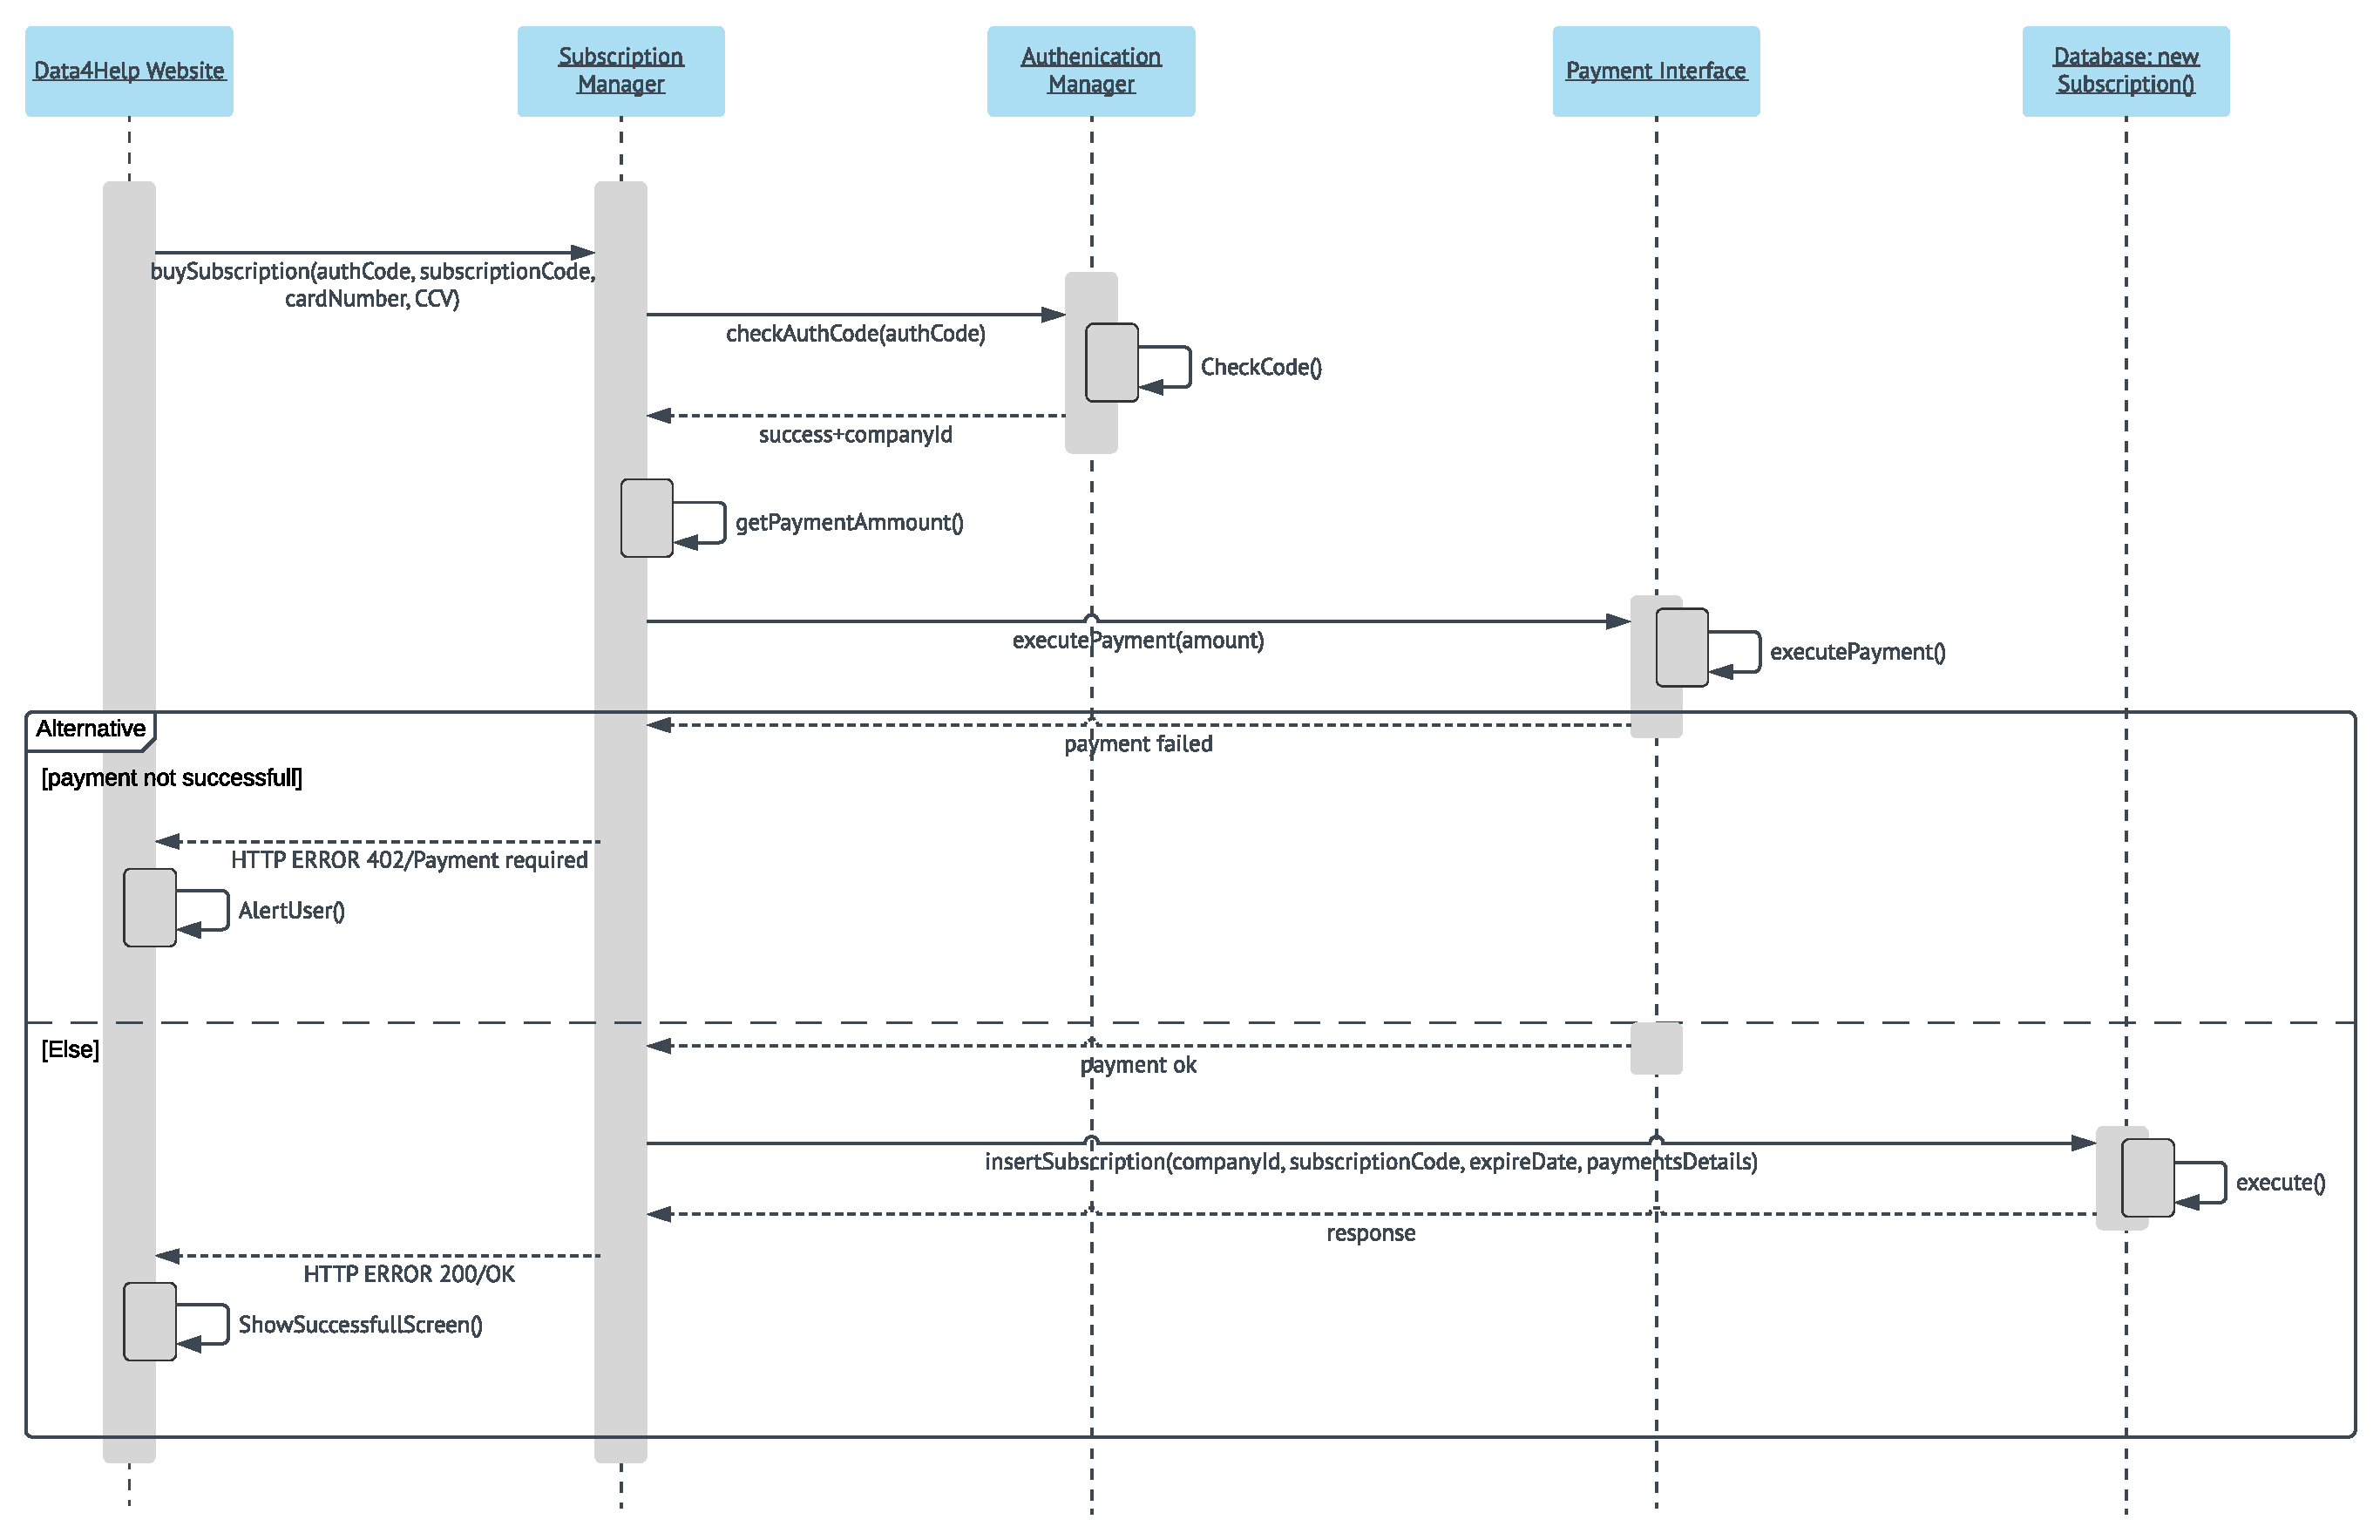
\includegraphics[width=\textwidth,height=\textheight,keepaspectratio]{assets/flowCharts/CompanyPaymentProcessing.pdf}
	\caption{Company Payment Processing Runtime View}
	\label{fig:CompanyPaymentProcessing}
\end{figure}


\subsubsection{Emergency Situation}
If a user is subscribed to the AutomatedSOS service, whenever the Individual Manager receives new data from the Mobile App, it also sends a checkUserThresholds request to the EmergencyManager, specifying the SSN of the individual and the health data received. Firstly the EmergencyManager checks if the user is subscribed to AutomatedSOS, if so, it checks the threshold for that specific user: in the case in which the data parameters are lower than the specified threshold, the EmergencyManager instantly sends a sendAmbulance request to the EmergencyInterface, which will contact the ambulance API and requests an ambulance for the person. To do so, in the request includes the user position. 
\begin{figure}[H]
	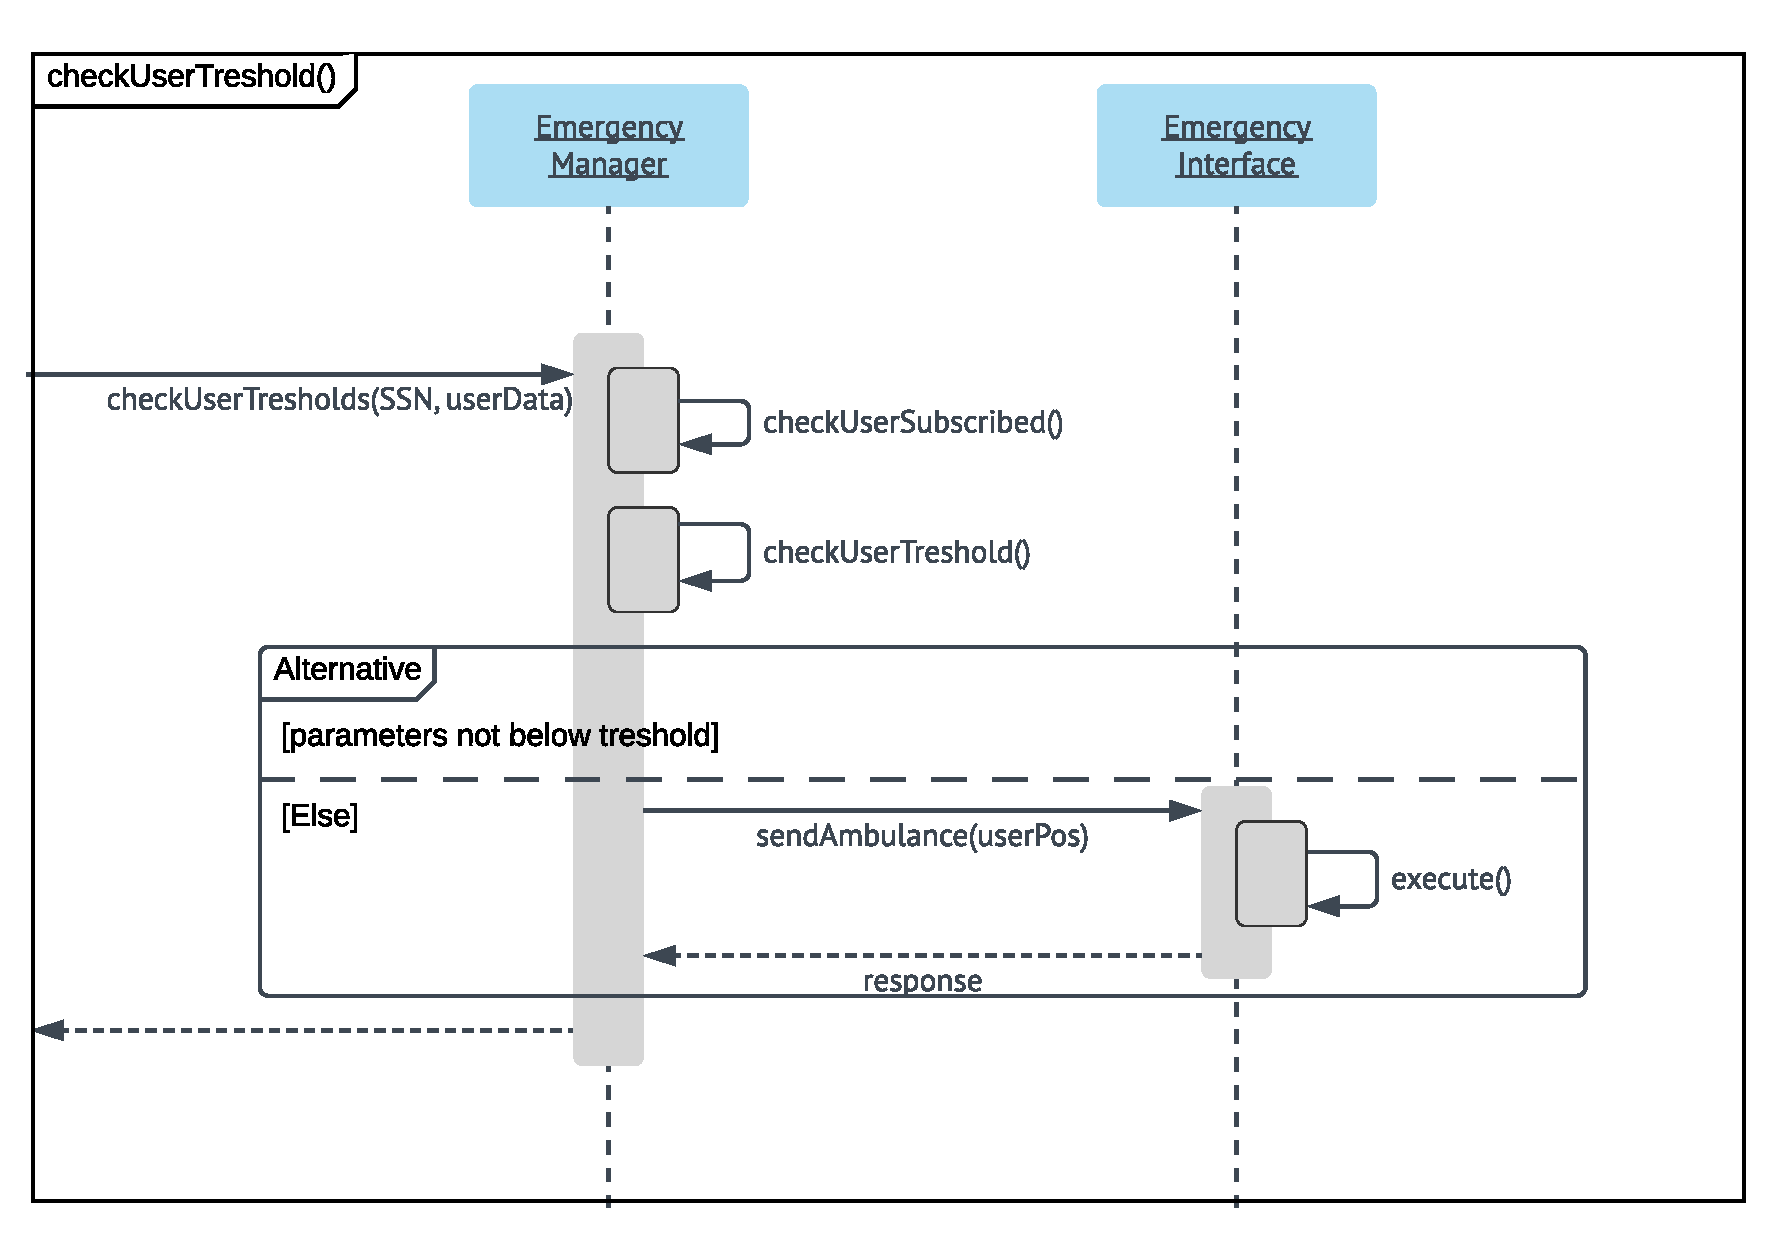
\includegraphics[width=\textwidth,height=\textheight,keepaspectratio]{assets/flowCharts/EmergencySituation.pdf}
	\caption{Emergency Situation Runtime View}
	\label{fig:EmergencySituation}
\end{figure}


\subsubsection{Run Organizer Adds New Race}
When a run organizer wants to add a new race using the Data4Help Mobile App, he goes to the corresponding section, fills information about the run and clicks on "Create new run".\\
The website sends a createNewRun request specifying the authToken and runData, the Authentication manager authenticates the user, and checks data consistency.
If data is consistent, the Run Manager goes on inserting the new run into the Track4Me database and returns a successfull response to the client, otherwise it returns an error and alerts the user.
\begin{figure}[H]
	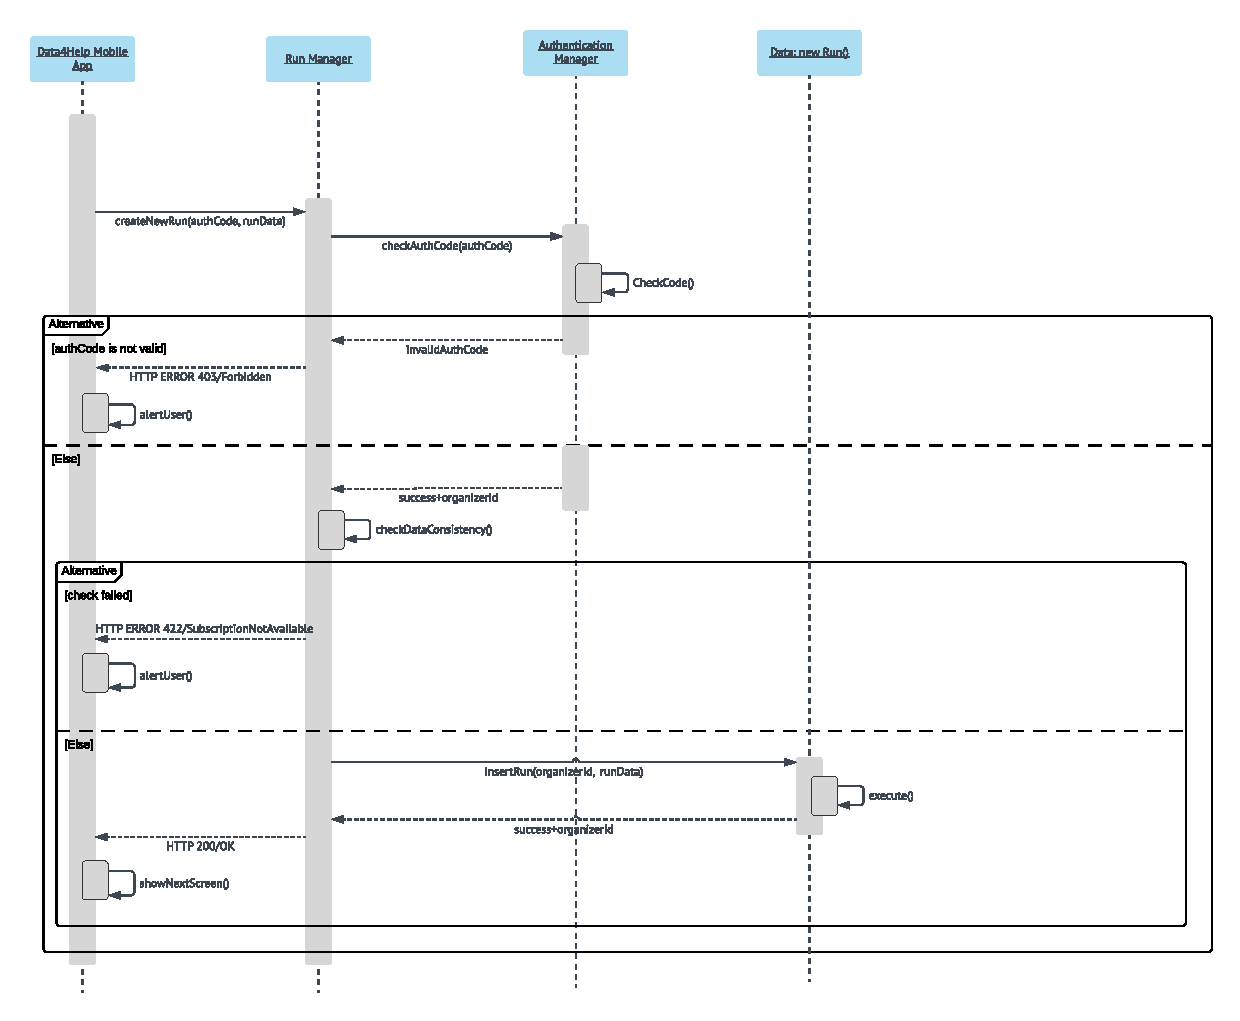
\includegraphics[width=\textwidth,height=\textheight,keepaspectratio]{assets/flowCharts/RunOrganizerAddsNewRace.pdf}
	\caption{Run Organizer Adds New Race Runtime View}
	\label{fig:RunOrganizerAddsNewRace}
\end{figure}



\subsubsection{Runner Subscription To A Race}
When a user of Data4Help wants to subscribe to a run, it must send a getRunList request containing its geographical position to the RunManager. \\
Firstly, the RunManager computes which races have their starting point 30km close to the runner position, then returns the mentioned list to the user. 
Then, the user chooses the run he wants to subscribe to and sends a subscribeUser request to the RunManager containing the authToken and the runId. \\
The user is authenticated by the Authentication Manager, if the sent authToken is correct, the RunManager goes on checking if the chosen race has already started.\\ If the race has already started, the Run Manager sends an error to the client, otherwise, adds the user to the runner lists sending an addUserToRun to the Run Manager(specifying the user SSN and the runId).\\

\begin{figure}[H]
	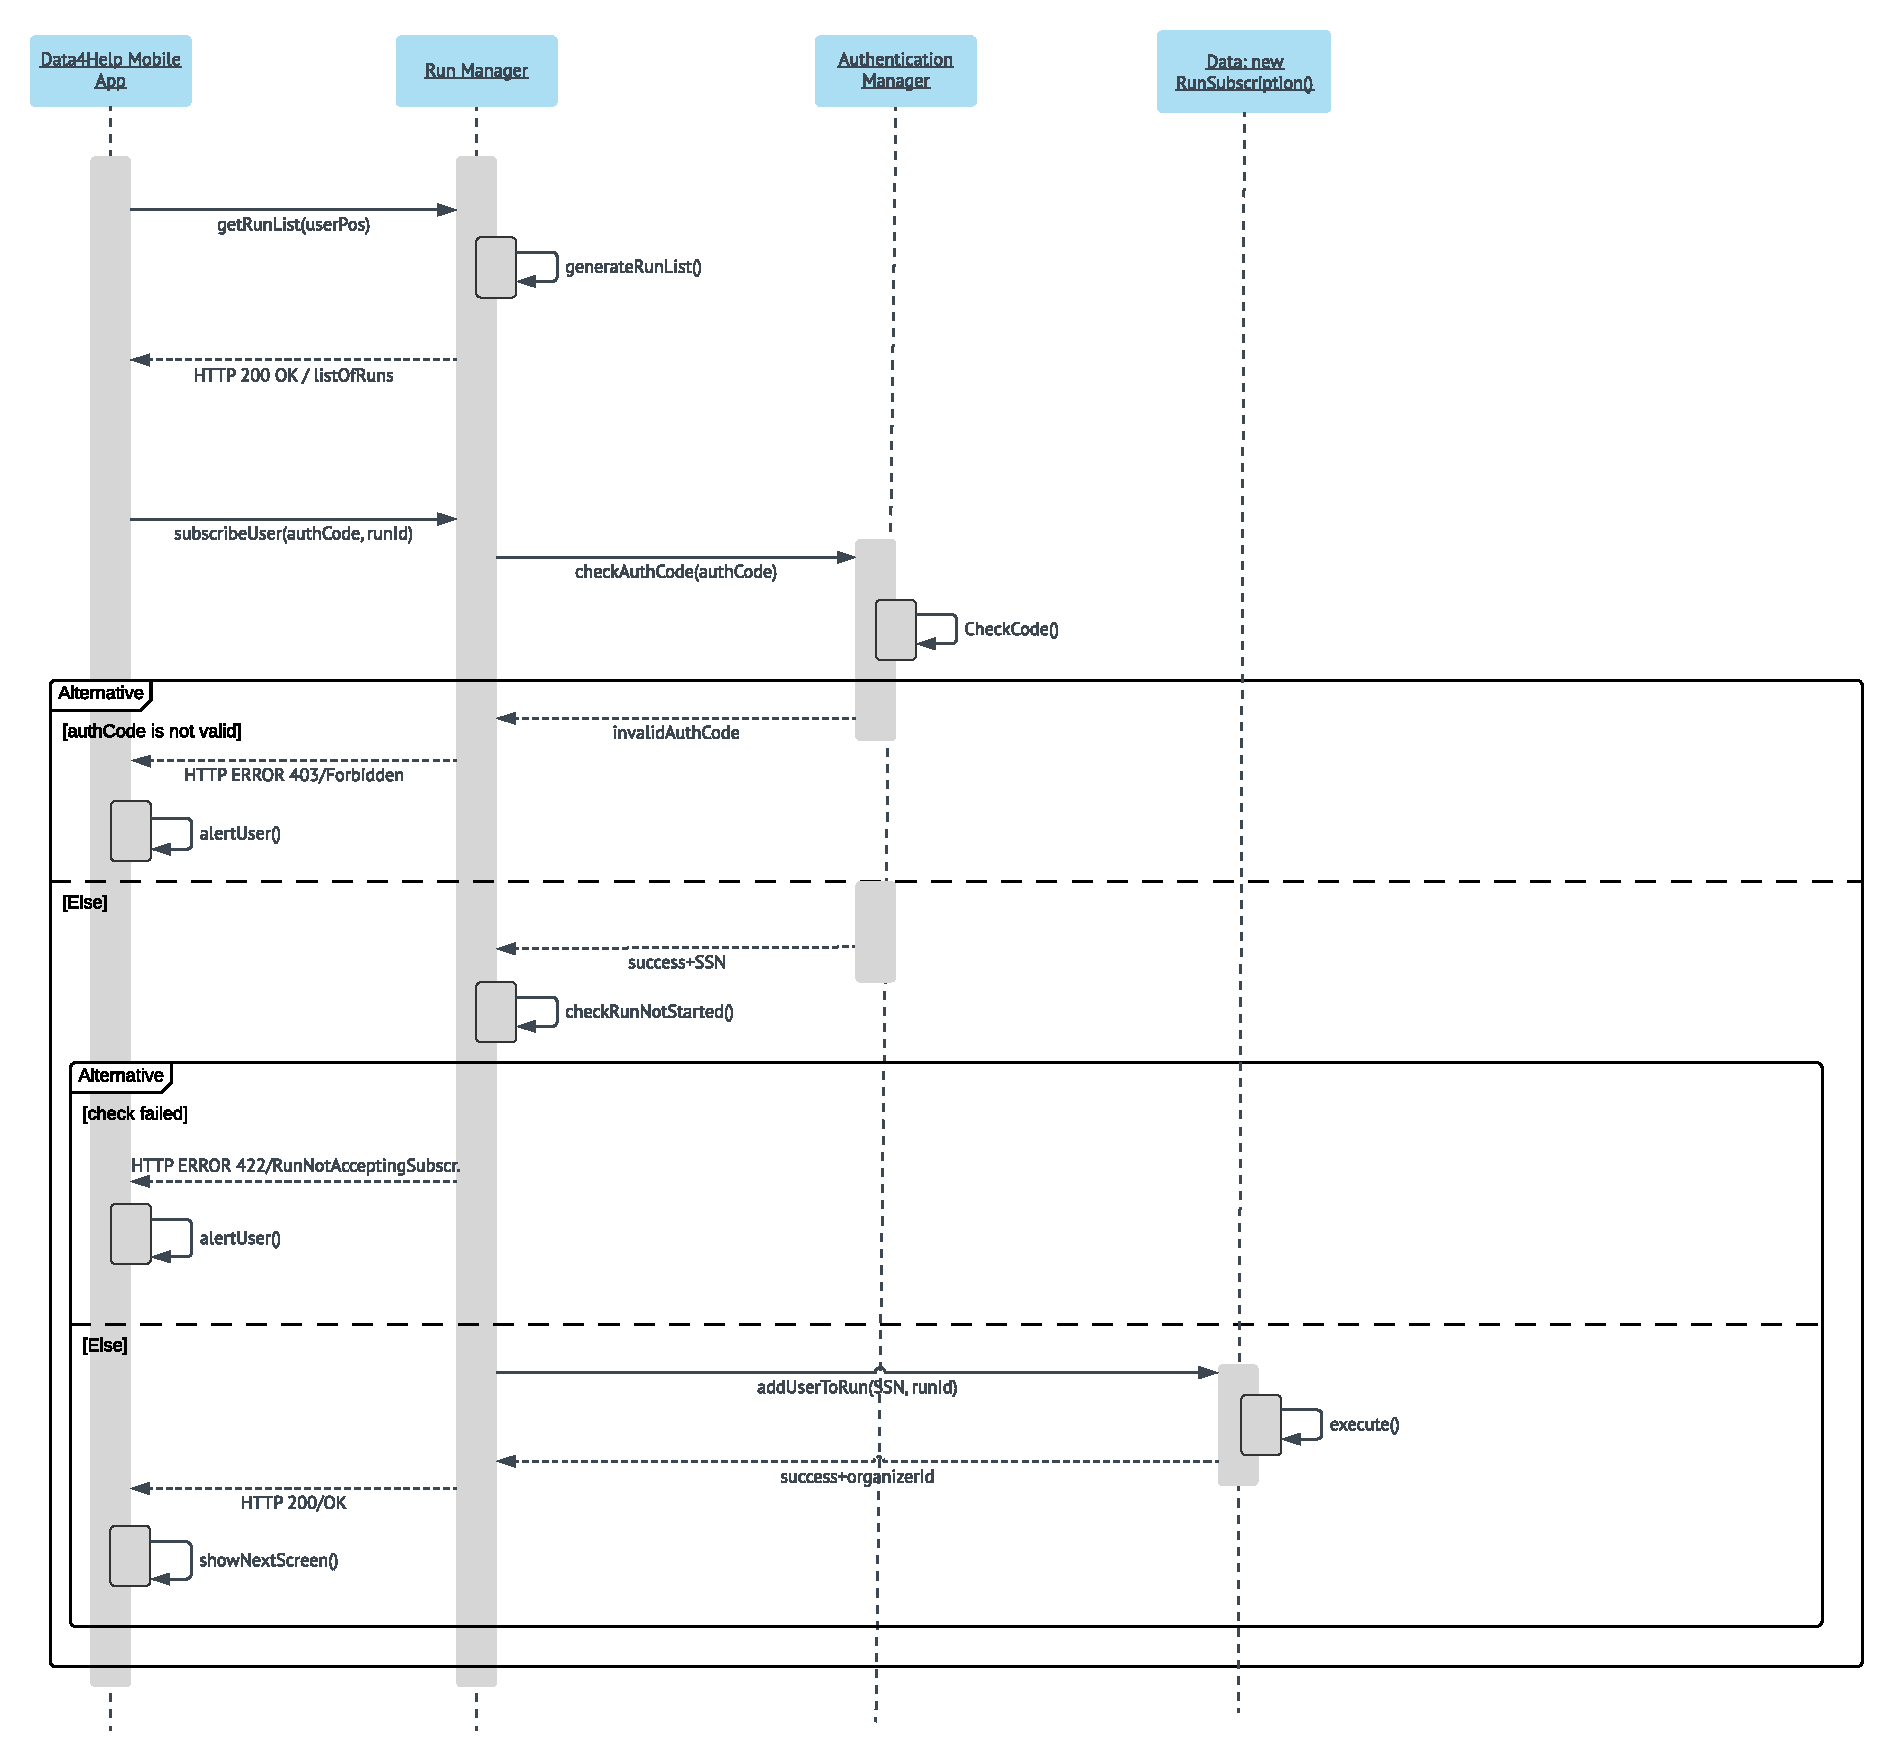
\includegraphics[width=\textwidth,height=\textheight,keepaspectratio]{assets/flowCharts/RunnerSubscriptionToARace.pdf}
	\caption{Runner Subscription To A Race Runtime View}
	\label{fig:RunnerSubscriptionToARace}
\end{figure}


\subsubsection{Spectator Of Run Request Run Position}
When a user wants to see the map of the runners of a run, he must request the runner positions to the RunManager.\\
The Mobile app sends an getRunnerPositions request specifiyng the code of the run followed to the RunManager that, after checking if the run is still active, get all the users position in run identifying them with the SSN.\\ Then, it sends a getUserPosFromDatetime request, specifying the runStartDatetime, it computes if the user has passed checkpoints (computeCheckPoint), eventually add the information of the user in a list. \\
Finally, the userList with the data about checkpoint passed and the geographical position is returned to the Mobile App, that shows in a map all runner positions.


\begin{figure}[H]
	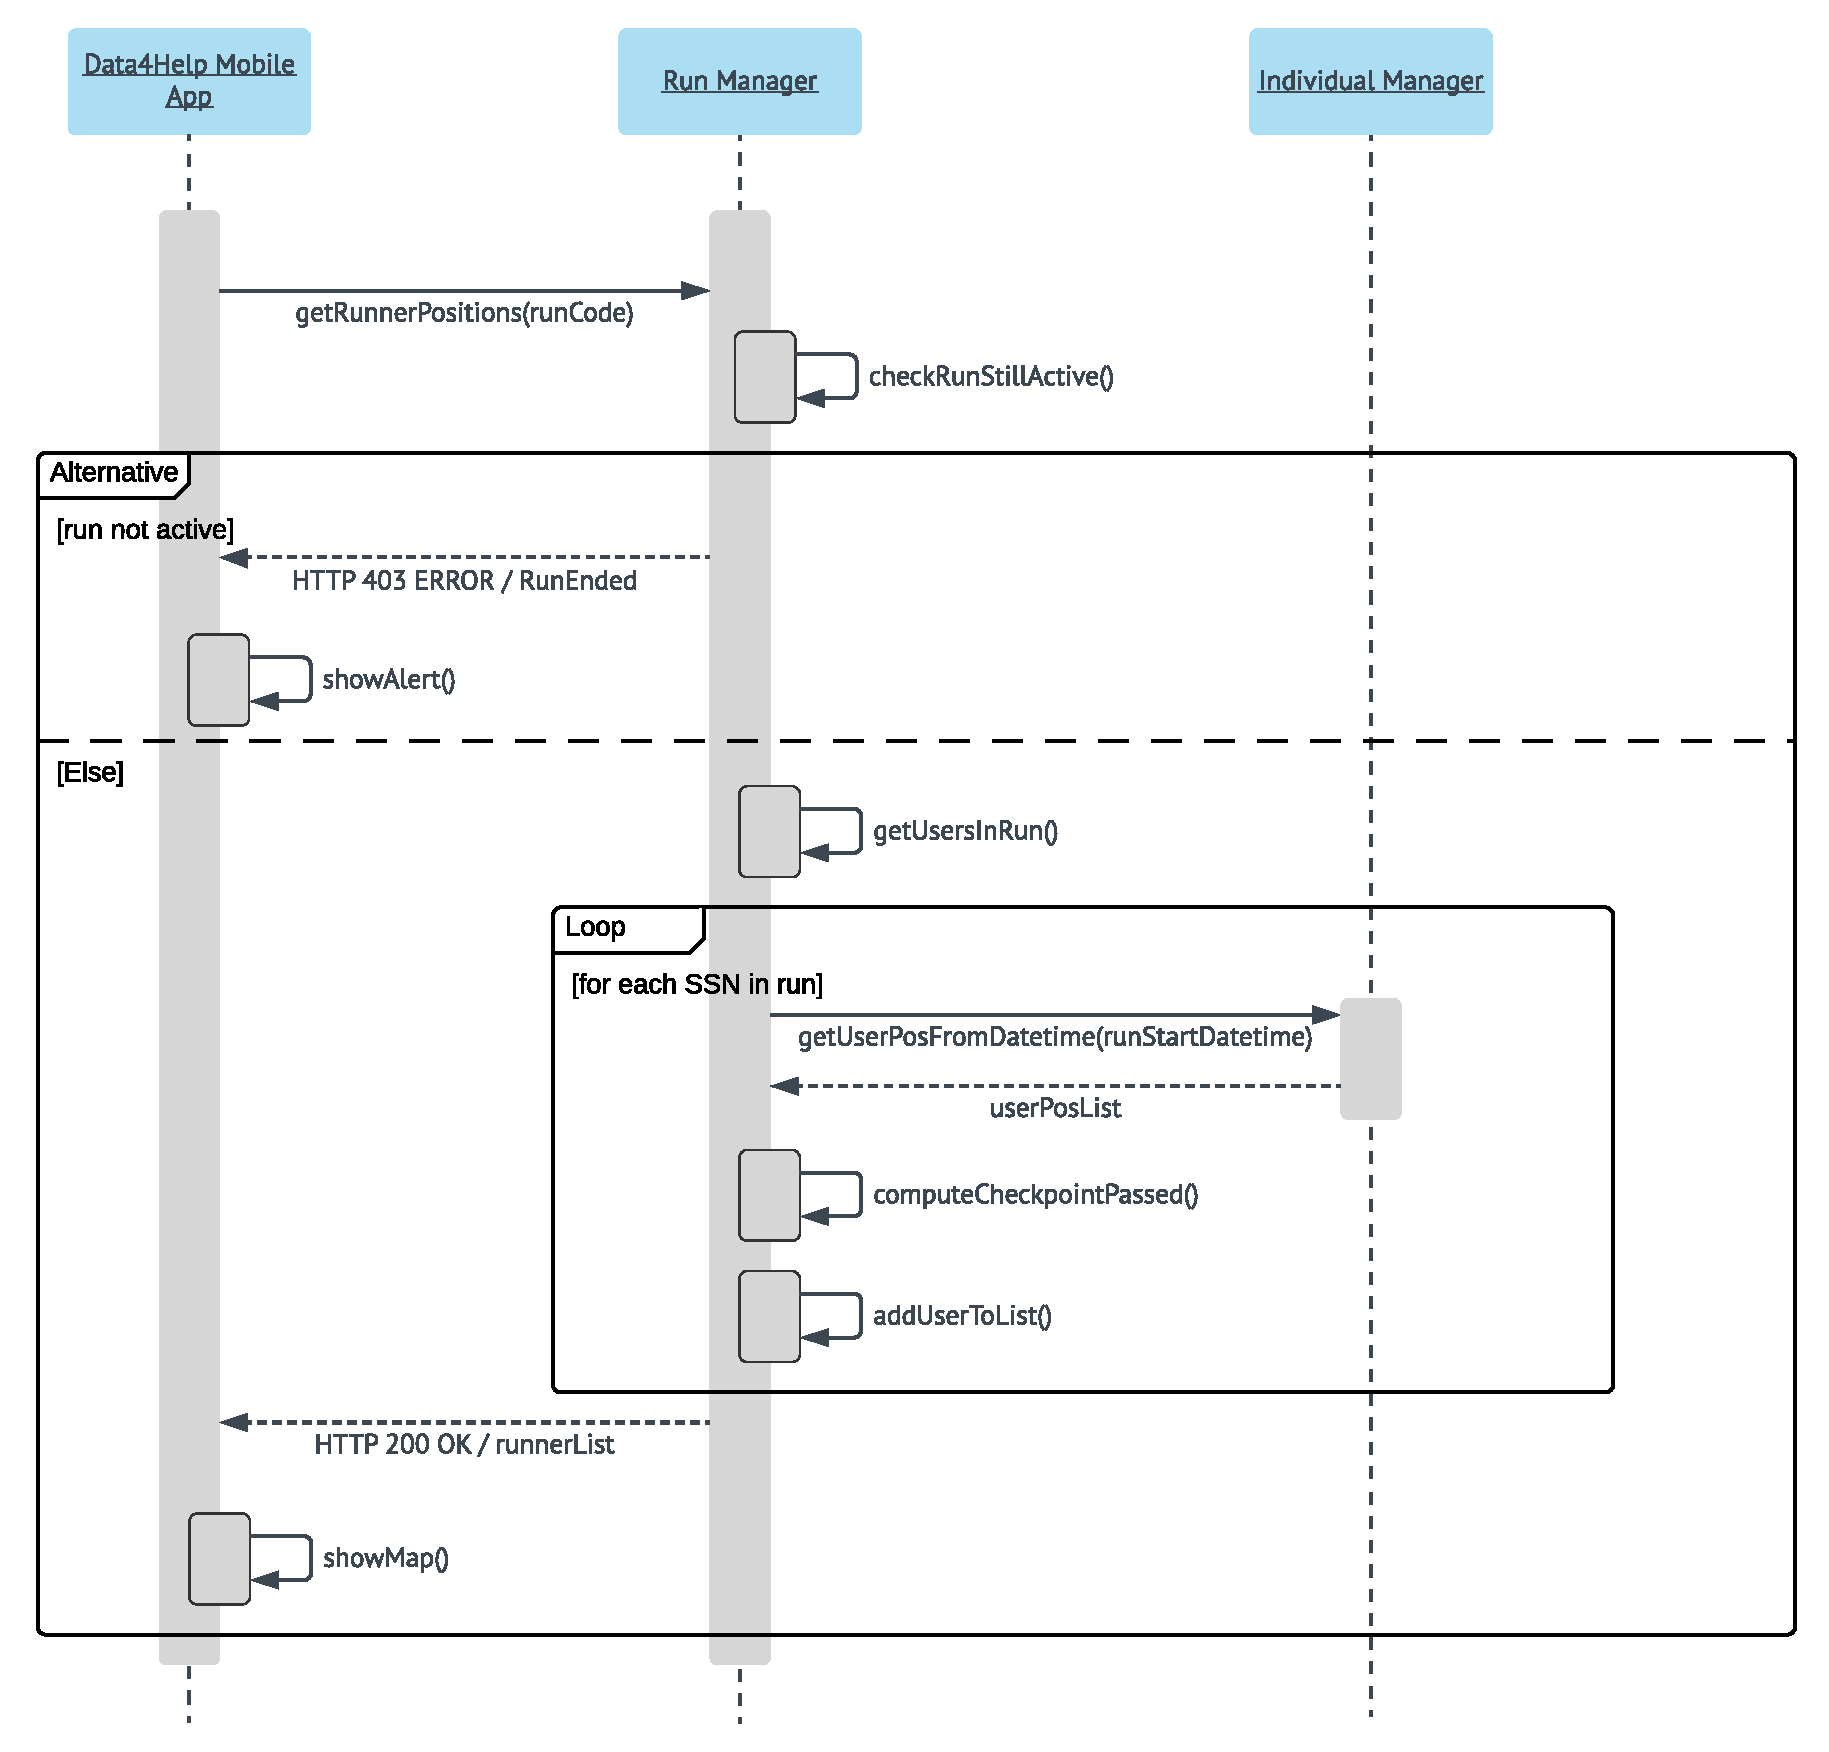
\includegraphics[width=\textwidth,height=\textheight,keepaspectratio]{assets/flowCharts/SpectatorOfRunRequestRunPosition.pdf}
	\caption{Spectator Of Run Request Run Position Runtime View}
	\label{fig:SpectatorOfRunRequestRunPosition}
\end{figure}